\documentclass{ansjournal}

\usepackage{microtype}                     % Improve typography
\usepackage{amsmath, mathtools}             % AMS Math extensions
\usepackage{booktabs}                      % Improved table spacing
\usepackage{siunitx}
\usepackage{breqn}
\usepackage{nicefrac}
\usepackage{multirow}
\usepackage{enumitem}
\usepackage{subcaption}
\usepackage{dblfloatfix}
\usepackage{color}
\usepackage{todonotes}
\usepackage{etoolbox}
\usepackage{listings}
\usepackage{color}
\usepackage{bbold}
\usepackage{breqn}

% Checkmarks
\usepackage{amssymb}% http://ctan.org/pkg/amssymb
\usepackage{pifont}% http://ctan.org/pkg/pifont
\newcommand{\cmark}{\ding{51}}%
\newcommand{\xmark}{\ding{55}}%

\newcommand{\code}[2]{
  \subsection*{#1}
  \lstinputlisting{#2}
}

\lstset{
  basicstyle=\footnotesize\ttfamily,
  columns=fullflexible,
  showstringspaces=false,
  commentstyle=\color{gray}\upshape,
  frame=single,
  xleftmargin=0.8in,
  xrightmargin=0.8in
}

\crefname{lstlisting}{Listing}{Listings}

% Patch to make equation autoref counter work
\makeatletter
\patchcmd\eq@setnumber{\stepcounter}{\refstepcounter}{}{%
  \errmessage{Patching \noexpand\eq@setnumber failed}%
}
\makeatother

\hypersetup{colorlinks=true,
  pdftitle={Multigroup Cross Section Generation with the OpenMC Monte Carlo Particle Transport Code},
  pdfauthor={William Boyd, Adam Nelson, Paul Romano, Samuel Shaner, Benoit Forget and Kord Smith}}

\title{Multigroup Cross Section Generation with the OpenMC Monte Carlo Particle Transport Code}

\author[a]{William Boyd\footnote{Email: \href{mailto:boyd.william.r@gmail.com}{boyd.william.r@gmail.com}}}
\author[b]{Adam Nelson}
\author[c]{Paul K. Romano}
\author[d]{Samuel Shaner\footnote{This author was a graduate research assistant at the Massachusetts Institute of Technology at the time this research was conducted.}}
\author[a]{Benoit Forget}
\author[a]{Kord Smith}

\affil[a]{Massachusetts Institute of Technology, Department of Nuclear Science
  and Engineering, 77 Massachusetts Avenue, Building 24, Cambridge,
  Massachusetts 02139}
\affil[b]{Naval Reactors, 1240 Isaac Hull Ave. SE, Washington Navy Yard, D.C. 20376}
\affil[c]{Argonne National Laboratory, Mathematics and Computer Science
  Division, 9700 South Cass Avenue, Lemont, Illinois 60439}
\affil[d]{Yellowstone Energy, 11631 Lanesborough Way, Farragut, Tennessee 37934}

%%%%%%%%%%%%%%%%%%%%%%%%%%%%%%%%%%%%%%%%%%%%%%%%%%%%%%%%%%%%%%%%%%%%%%%%%%%%%%%
\abstractText{High-fidelity deterministic transport codes require highly accurate multigroup cross sections (MGXS). Monte Carlo is increasingly cited as a reactor-agnostic approach to MGXS generation since it is unconstrained by the engineering-based approximations that limit the applicability of deterministic MGXS generation tools. This paper introduces a new framework that uses the OpenMC Monte Carlo code to generate MGXS for use in multigroup transport codes. The \texttt{openmc.mgxs} module is built atop OpenMC's Python API to process tally data output by the OpenMC executable. This paper validates the module to generate MGXS that enable the multigroup OpenMOC transport code to compute eigenvalues to within 50 pcm and fission rates to within 1\% of reference solutions for two heterogeneous pressurized water reactor benchmarks.}

%%%%%%%%%%%%%%%%%%%%%%%%%%%%%%%%%%%%%%%%%%%%%%%%%%%%%%%%%%%%%%%%%%%%%%%%%%%%%%%

\keywordsText{Monte Carlo neutron transport, multigroup cross section generation, OpenMC}

\begin{document}

\maketitle

%%%%%%%%%%%%%%%%%%%%%%%%%%%%%%%%%%%%%%%%%%%%%%%%%%%%%%%%%%%%%%%%%%%%%%%%%%%%%%%
\section{Introduction}
\label{sec:intro}
%%%%%%%%%%%%%%%%%%%%%%%%%%%%%%%%%%%%%%%%%%%%%%%%%%%%%%%%%%%%%%%%%%%%%%%%%%%%%%%

The past two decades have seen growing interest in Monte Carlo (MC) as a means to generate multi-group cross section (MGXS) libraries. Most MC-based MGXS generation schemes to date focus on generating few-group constants for coarse mesh diffusion codes. These schemes aim to improve the accuracy of standard diffusion codes for analysis of atypical core configurations for which the simplifications made by multilevel deterministic MGXS generation methods are not necessarily applicable. These efforts replace the separate resonance self-shielding and deterministic lattice physics calculation steps in multistep approaches with fully detailed MC calculations of each assembly to compute the few-group constants needed by whole-core diffusion codes. The widely used Serpent code\cite{leppanen2015serpent} has led this trend over the past decade, and a few authors have applied the MCNP\cite{pounders2006stochastically} and McCARD\cite{shim2008generation} codes in a similar fashion. This paper presents new capabilities introduced in the OpenMC\cite{romano2015openmc} particle transport code for multi-group cross section generation for fine-mesh multi-group neutron transport applications.

This paper is organized as follows. \cref{sec:mg-theory} summarizes the key multi-group constants required by deterministic multi-group codes. \cref{sec:mgxs-mc} details the mathematical formulation for stochastic integration of each of the multi-group constants currently computable by OpenMC. \cref{sec:openmc} highlights the core OpenMC features that provide the foundation for the \texttt{openmc.mgxs} module for MGXS generation introduced in \cref{sec:design}. \cref{sec:validate} uses the OpenMOC\cite{boyd2014openmoc} multi-group transport code to validate the MGXS generated by OpenMC. \cref{sec:conclusions} summarizes the conclusions.

%%%%%%%%%%%%%%%%%%%%%%%%%%%%%%%%%%%%%%%%%%%%%%%%%%%%%%%%%%%%%%%%%%%%%%%%%%%%%%%%
\section{Multi-Group Transport Methods}
\label{sec:mg-theory}

A key trend in recent years has been the steady progress toward full-core neutron transport-based reactor analysis tools. Transport-based methods for reactor physics apply a variety of approximations to solve the following form of the steady-state Boltzmann transport equation,

\begin{dmath}
\label{eqn:transport-ce}
\mathbf{\Omega} \cdot \nabla \psi(\mathbf{r},\mathbf{\Omega},E) + \Sigma_{t}(\mathbf{r},E)\psi(\mathbf{r},\mathbf{\Omega},E) = \int\displaylimits_{0}^{\infty}\int\displaylimits_{4\pi} \Sigma_{s}(\mathbf{r},{\mathbf{\Omega'}\rightarrow\mathbf{\Omega}},{E'\rightarrow E}) \psi(\mathbf{r},\mathbf{\Omega'},E') \mathrm{d}\mathbf{\Omega'} \mathrm{d}E' + \frac{1}{k_{\textrm{eff}}}\int\displaylimits_{0}^{\infty}\int\displaylimits_{4\pi} \nu\Sigma_{f}(\mathbf{r},{\mathbf{\Omega'}\rightarrow \mathbf{\Omega}},{E'\rightarrow E})\psi(\mathbf{r},\mathbf{\Omega'},E') \mathrm{d}\mathbf{\Omega'} \mathrm{d}E'\,,
\end{dmath}

\noindent which is integro-differential in the neutron angular flux $\psi(\mathbf{r},\mathbf{\Omega},E)$ in space $\mathbf{r}$, direction of travel $\mathbf{\Omega}$, and energy $E$. The equation depends on the macroscopic total, scattering, and fission production cross sections $\Sigma_{t}$, $\Sigma_{s}$, and $\nu\Sigma_{f}$, respectively, and the eigenvalue $k_{\textrm{eff}}$ of the critical system.

The accurate determination of the neutron flux is challenged primarily by the complicated energy structure of the cross sections. Monte Carlo transport methods are able to exactly treat the energy dependence in \cref{eqn:transport-ce}\footnote{The treatment is only as exact as the uncertainties in measured nuclear cross section data will permit.}, but they are computationally burdensome and impractical for routine nuclear reactor analysis. Deterministic methods do not make use of continuous energy cross sections and instead rely on multi-group constants as a result of several simplifying approximations to \cref{eqn:transport-ce}, including energy and spatial discretization, angular expansion of the scattering kernel, and an isotropic fission source. The deterministic OpenMOC transport code used in this paper solves the following form of the multi-group transport equation,

\begin{equation}
\label{eqn:transport-mg}
\mathbf{\Omega} \cdot \nabla \psi_{g}(\mathbf{r},\mathbf{\Omega}) + \Sigma_{tr,g}\psi_{g}(\mathbf{r},\mathbf{\Omega}) = \frac{1}{4\pi} \sum_{g'=1}^{G} \Sigma_{s,k,g' \rightarrow g}\phi_{g'}(\mathbf{r}) + \frac{\chi_{k,g}}{4\pi k_{\textrm{eff}}}\sum_{g'=1}^{G} \nu\Sigma_{f,k,g'}\phi_{g'}(\mathbf{r})\,,
\end{equation}

\noindent where the subscript $k$ corresponds to the discretized spatial mesh cell $k$ and energy group $g \in \left\{1, 2, \ldots, G\right\}$ spans a range of energies from $\left[E_{g}, E_{g-1}\right]$. This form of the equation depends on the angular- and energy-integrated scalar flux $\phi_g$. The multi-group transport-corrected total cross section $\Sigma_{tr,k,g}$, isotropic group-to-group scattering matrix $\Sigma_{s,k,g'\rightarrow g}$, fission production cross section $\nu\Sigma_{f,k,g}$ and fission energy spectrum $\chi_{k,g}$ must be precomputed and supplied as parameters to multi-group codes that solve this form of the multi-group transport equation.

%%%%%%%%%%%%%%%%%%%%%%%%%%%%%%%%%%%%%%%%%%%%%%%%%%%%%%%%%%%%%%%%%%%%%%%%%%%%%%%
\section{MGXS Generation with Monte Carlo}
\label{sec:mgxs-mc}
%%%%%%%%%%%%%%%%%%%%%%%%%%%%%%%%%%%%%%%%%%%%%%%%%%%%%%%%%%%%%%%%%%%%%%%%%%%%%%%


%%%%%%%%%%%%%%%%%%%%%%%%%%%%%%%%%%%%%%%%%%%%%%%%%%%
\subsection{Tally Types Needed for MGXS Generation}
\label{subsec:tally-types}

This section describes how multi-group cross sections may be computed using stochastic integration. In particular, this section outlines the types of OpenMC tallies needed to generate MGXS -- including the scores, filters and estimators for each tally -- and the arithmetic combinations used to combine different tallies.

%%%%%%%%%%%%%%%%%%%%%%%%%%%%%%%%%%%%%%
\subsubsection{Inner Product Notation}
\label{subsubsec:tally-types-notation}

The following sections use angle bracket notation $\langle \cdot , \cdot \rangle$ to represent inner products in phase space. This may correspond to integrals over incoming and/or outgoing energy, space, and angle. Using this notation, a tally estimator for reaction rate $x$ is represented as follows: 

\begin{equation}
\label{eqn:inner-prod}
\langle \Sigma_x, \psi \rangle = \int_{V} \int_{S} \int_{E} \Sigma_{x}(\mathbf{r},E)\psi(\mathbf{r},E,\mathbf{\Omega}) \mathrm{d}E\mathrm{d}\mathbf{\Omega}\mathrm{d}\mathbf{r}
\end{equation}

\noindent This notation is specialized throughout this section with subscripts to indicate the subsets of phase space that are integrated over in the inner product. In particular, subscript $k$ refers to a volume integral over $V_{k}$ for some region of space $k$ for spatial homogenization, while subscript $g$ corresponds to an integral over energies with $E \in [E_{g}, E_{g-1}]$ for energy condensation. For example, the microscopic reaction rate for reaction $x$ by nuclide $i$ is denoted as:

\begin{equation}
\label{eqn:angle-rxn-rate}
\langle \sigma_{x,i}, \psi \rangle_{k,g} = \int_{\mathbf{r} \in V_{k}} \int_{4\pi} \int_{E_{g}}^{E_{g-1}} \sigma_{x,i}(\mathbf{r},E)\psi(\mathbf{r},E,\mathbf{\Omega}) \mathrm{d}E\mathrm{d}\mathbf{\Omega}\mathrm{d}\mathbf{r}
\end{equation}

\noindent The inner product of a function with unity, such as the spatially-homogenized and energy-integrated flux is denoted by:

\begin{equation}
\label{eqn:angle-flux}
\langle \psi \rangle_{k,g} \equiv \langle \psi, \mathbb{1} \rangle_{k,g} = \int_{\mathbf{r} \in V_{k}} \int_{4\pi} \int_{E_{g}}^{E_{g-1}} \psi(\mathbf{r},E,\mathbf{\Omega}) \mathrm{d}E\mathrm{d}\mathbf{\Omega}\mathrm{d}\mathbf{r}
\end{equation}

%Finally, the superscripts $a$ and $t\ell$ are given to those inner products computed with analog and track-length estimators, respectively -- \textit{i.e.}, $\langle \cdot,\cdot \rangle^{a}$ is an analog tally estimator and $\langle \cdot,\cdot \rangle^{t\ell}$ is a track-length tally estimator of the corresponding inner products.

%%%%%%%%%%%%%%%%%%%%%%%%%%%%%%%%%%%%%%%%%%%%%%
\subsubsection{General Reaction Cross Section}
\label{subsubsec:tally-types-gen-xs}

A general spatially-homogenized and energy condensed macroscopic multi-group cross section for reaction $x$, spatial zone $k$ and energy group $g$ is simply the ratio of the group-wise reaction rates $\langle \Sigma_{x}, \psi \rangle_{k,g}$ and fluxes $\langle \psi \rangle_{k,g}$:

\begin{equation}
\label{eqn:general-macro}
\hat{\Sigma}_{x,k,g} = \frac{\langle \Sigma_{x}, \psi \rangle_{k,g}}{\langle \psi \rangle_{k,g}}
\end{equation}

\noindent Likewise, a microscopic MGXS for nuclide $i$ can be computed as follows:

\begin{equation}
\label{eqn:general-micro}
\hat{\sigma}_{x,i,k,g} = \frac{\langle \sigma_{x,i}, \psi \rangle_{k,g}}{\langle \psi \rangle_{k,g}}
\end{equation}

These estimators are used for reaction types which are only dependent on the incoming energy of a neutron, such as total and radiative capture reactions.

%%%%%%%%%%%%%%%%%%%%%%%%%%%%%%%%%%%
\subsubsection{Total Cross Section}
\label{subsubsec:tally-types-tot-xs}

The total macroscopic cross section $\Sigma_{t}$ is a special case of \autoref{eqn:general-micro}, with the total collision rate substituted into the numerator:

\begin{equation}
\label{eqn:total-macro}
\hat{\Sigma}_{t,k,g} = \frac{\langle \Sigma_{t}, \psi \rangle_{k,g}}{\langle \psi \rangle_{k,g}}
\end{equation}

A transport correction is often used to incorporate anisotropic scattering effects into the transport equation with an isotropic scattering kernel. An expression for the in-scatter approximation \cite{yamamoto2008simplified} to the transport correction is computed with an OpenMC tally for the first Legendre scattering moment:

\begin{equation}
\label{eqn:sigs1}
\langle \Sigma_{s1}, \psi \rangle_{k,g'\rightarrow g} = \int_{\mathbf{r} \in V_{k}} \int_{4\pi} \int_{E_{g}}^{E_{g-1}} \int_{E_{g'}}^{E_{g'-1}} \Sigma_{s1}(\mathbf{r},E'\rightarrow E)\psi(\mathbf{r},E',\mathbf{\Omega}) \mathrm{d}E'\mathrm{d}E\mathrm{d}\mathbf{\Omega}\mathrm{d}\mathbf{r}
\end{equation}

\noindent An analog estimator must be used in OpenMC since the tally includes an integral over the outgoing neutron energy. The spatially-homogenized and energy condensed transport-corrected total cross section is computed by summing over all incoming energy groups:

\begin{equation}
\label{eqn:transport-corr-macro}
\hat{\Sigma}_{tr,k,g} = \displaystyle\sum\limits_{g'=1}^{G} \langle{\Sigma_{s1}, \psi \rangle_{k,g'\rightarrow g}}
\end{equation}

\noindent The transport correction is then subtracted from the group-wise total collision rate and normalized by the flux to compute the transport-corrected total cross section:

\begin{equation}
\label{eqn:sigt-transport-macro}
\hat{\tilde{\Sigma}}_{t,k,g} = \frac{\langle \Sigma_{t}, \psi \rangle_{k,g} - \hat{\Sigma}_{tr,k,g}}{\langle \psi \rangle_{k,g}}
\end{equation}

Since the transport correction must be computed using an analog estimator, the total collision and flux in \autoref{eqn:sigt-transport-macro} must also be computed with analog estimators.

%%%%%%%%%%%%%%%%%%%%%%%%%%%%%%%%%%%
\subsubsection{Multiplicity Matrix}
\label{subsubsec:tally-types-mult-mat}

The multiplicity is calculated as

\begin{equation}
\langle \upsilon \sigma_{s,g'\rightarrow g} \phi \rangle = \int_{r \in D} dr \int_{4\pi} d\Omega' \int_{E_{g'}}^{E_{g'-1}} dE' \int_{4\pi} d\Omega \int_{E_g}^{E_{g-1}} dE \; \sum_i \upsilon_i \sigma_i (r, E' \rightarrow E, \Omega' \cdot \Omega) \psi(r, E', \Omega') 
\end{equation}

\begin{equation}
\langle \upsilon \sigma_{s,g'\rightarrow g} \phi \rangle = \int_{r \in D} dr \int_{4\pi} d\Omega' \int_{E_{g'}}^{E_{g'-1}} dE' \int_{4\pi} d\Omega \int_{E_g}^{E_{g-1}} dE \; \sum_i \upsilon_i \sigma_i (r, E' \rightarrow E, \Omega' \cdot \Omega) \psi(r, E', \Omega')
\end{equation}

\begin{equation}
\langle \sigma_{s,g'\rightarrow g} \phi \rangle = \int_{r \in D} dr \int_{4\pi} d\Omega' \int_{E_{g'}}^{E_{g'-1}} dE' \int_{4\pi} d\Omega \int_{E_g}^{E_{g-1}} dE \; \sum_i \upsilon_i \sigma_i (r, E' \rightarrow E, \Omega' \cdot \Omega) \psi(r, E', \Omega') \\
\end{equation}

\begin{equation}
\upsilon_{g'\rightarrow g} = \frac{\langle \upsilon \sigma_{s,g'\rightarrow g} \rangle}{\langle \sigma_{s,g'\rightarrow g} \rangle}
\end{equation}

\noindent where $\upsilon_i$ is the multiplicity for the $i^{th}$ reaction.


%%%%%%%%%%%%%%%%%%%%%%%%%%%%%%%%%%%%%%%%%%%%%
\subsubsection{Scattering Probability Matrix}
\label{subsubsec:tally-types-scatt-prob-mat}


%%%%%%%%%%%%%%%%%%%%%%%%%%%%%%%%%
\subsubsection{Scattering Matrix}
\label{subsubsec:tally-types-scatt-mat}

The isotropic scattering matrix is computed with an inner product of scattering reactions over both incoming and outgoing energies. An analog estimator must be used since the integral is dependent on the neutron's outgoing energy. Similar to the first Legendre moment in \autoref{eqn:sigs1}, the isotropic scattering moment is given by the following expression:

\begin{equation}
\label{eqn:sigs0}
\langle \Sigma_{s0}, \psi \rangle_{k,g'\rightarrow g} = \int_{\mathbf{r} \in V_{k}} \int_{4\pi} \int_{E_{g}}^{E_{g-1}} \int_{E_{g'}}^{E_{g'-1}} \Sigma_{s0}(\mathbf{r},E'\rightarrow E)\psi(\mathbf{r},E,\mathbf{\Omega}) \mathrm{d}E'\mathrm{d}E\mathrm{d}\mathbf{\Omega}\mathrm{d}\mathbf{r}
\end{equation}

\noindent The isotropic scattering matrix is then:

\begin{equation}
\label{eqn:scatt-macro}
\hat{\Sigma}_{s,k,g'\rightarrow g} = \frac{\langle \Sigma_{s0}, \psi \rangle_{k,g'\rightarrow g}}{\langle \psi \rangle_{k,g'}}
\end{equation}

\noindent The transport correction in \autoref{eqn:transport-corr-macro} can be applied by subtracting it from the diagonal elements in the matrix to compute the transport-corrected scattering matrix:

\begin{equation}
\label{eqn:scatt-trans-macro}
\hat{\tilde{\Sigma}}_{s,k,g'\rightarrow g} = \frac{\langle \Sigma_{s0}, \psi \rangle_{k,g'\rightarrow g} - \delta_{g,g'} \hat{\Sigma}_{tr,k,g}}{\langle \psi \rangle_{k,g'}}
\end{equation}

%To incorporate the effect of neutron multiplication from $(n,xn)$ reactions in the above relation, the nu parameter can be set to `True`.

An alternative ``consistent'' form of the scattering matrix can be computed as the product of the scatter cross section and group-to-group scattering probabilities. Unlike the formulation in \autoref{eqn:scatt-macro}, the consistent formulation is computed from the groupwise scattering cross section which uses a track-length estimator. This ensures that reaction rate balance is exactly preserved with a total cross section (\autoref{eqn:total-macro} computed using a tracklength estimator.

For a scattering probability matrix $P_{s,\ell,g'\rightarrow g}$ and scattering cross section $\sigma_s (r, E)$ for incoming energy group $[E_{g'},E_{g'-1}]$ and outgoing energy group $[E_g,E_{g-1}]$, the Legendre scattering moments are calculated as:

\begin{equation}
\label{eqn:scatt-mat-consistent}
\Sigma_{s,\ell,g'\rightarrow g} = \sigma_s (r, E) \times P_{s,\ell,g'\rightarrow g}
\end{equation}

To incorporate the effect of neutron multiplication from $(n,xn)$ reactions ...

\begin{equation}
\label{eqn:nuscatt-mat-consistent}
\sigma_{s,\ell,g'\rightarrow g} = \upsilon_{g'\rightarrow g} \times \sigma_s (r, E) \times P_{s,\ell,g'\rightarrow g}
\end{equation}

Add discussion about consistent scattering formulation ... and about Legendre moments ...

%%%%%%%%%%%%%%%%%%%%%%%%%%%%%%%%%%%%%%%%%%%%%%%%
\subsubsection{Fission Production Cross Section}
\label{subsubsec:tally-types-fiss-prod}

The fission product macroscopic cross section $\nu\Sigma_{f}$ may be treated as a special case of \autoref{eqn:general-micro}, with estimators for the fission production rate and flux:

\begin{equation}
\label{eqn:nu-fiss-macro}
\nu\hat{\Sigma}_{f,k,g} = \frac{\langle \nu\Sigma_{f}, \psi \rangle_{k,g}}{\langle \psi \rangle_{k,g}}
\end{equation}

%%%%%%%%%%%%%%%%%%%%%%%%%%%%%%%%%%%%%%%
\subsubsection{Fission Energy Spectrum}
\label{subsubsec:tally-types-chi}

Unlike the fission production cross section, the fission spectrum is dependent on the outgoing neutron energy and must be computed with analog estimators. The fission production matrix from group $g'$ into group $g$ is given by the following inner product:

\begin{equation}
\label{eqn:nu-fiss-energies}
\langle \nu\Sigma_{f}, \psi \rangle_{k,g'\rightarrow g} = \int_{\mathbf{r} \in V_{k}} \int_{4\pi} \int_{E_{g}}^{E_{g-1}} \int_{E_{g'}}^{E_{g'-1}} \nu\Sigma_{f}(\mathbf{r},E'\rightarrow E)\psi(\mathbf{r},E,\mathbf{\Omega}) \mathrm{d}E'\mathrm{d}E\mathrm{d}\mathbf{\Omega}\mathrm{d}\mathbf{r}
\end{equation}

\noindent The fission spectrum can then be computed from this tally by summing over incoming and outgoing energy groups:

\begin{equation}
\label{eqn:chi}
\hat{\chi}_{k,g} = \frac{\displaystyle\sum\limits_{g'=1}^{G} \langle \nu\Sigma_{f}, \psi \rangle_{k,g'\rightarrow g}}{\displaystyle\sum\limits_{g=1}^{G} \displaystyle\sum\limits_{g'=1}^{G} \langle \nu\Sigma_{f}, \psi \rangle_{k,g'\rightarrow g}}
\end{equation}

\noindent This expression for the fission spectrum will result in a normalized discrete probability distribution for the energy of neutrons emitted from fission.

%%%%%%%%%%%%%%%%%%%%%%%%%%%%%%%%%%%%%%%%
\subsubsection{Delayed Neutron Fraction}
\label{subsubsec:tally-types-beta}

%%%%%%%%%%%%%%%%%%%%%%%%%%%%%%%%%%%%%%%%%%%%%%%%%%%%
\subsubsection{Delayed Neutron Precursor Decay Rate}
\label{subsubsec:tally-types-lambda}

%%%%%%%%%%%%%%%%%%%%%%%%%%%%%%%%%%%%%%%%%%%%%%%%%%%%%%%%
\subsubsection{Delayed Fission Production Cross Section}
\label{subsubsec:tally-types-delay-fiss-prod}

%%%%%%%%%%%%%%%%%%%%%%%%%%%%%%%%
\subsubsection{Inverse Velocity}
\label{subsubsec:tally-types-inv-vel}


%%%%%%%%%%%%%%%%%%%%%%%%%%%%%%%%%%%%%%%%%%%%%%%%%%%
\subsection{Summary}
\label{subsec:tally-types-summary}

The tallies needed to generate MGXS libraries were outlined in detail in the preceding sections, and are summarized in \autoref{tab:tally-types}. The scores and filters correspond to the notation used by the OpenMC code to describe the scoring function and integration bounds. The energy group structure for energy condensation is specified by \texttt{energy} and/or \texttt{energyout} filters in the table. A material, cell, universe or mesh domain is specified by an appropriate filter for spatial homogenization.

\begin{table}[h!]
  \centering
  \caption[Tally types for MGXS generation]{The types of tallies used in MGXS generation with OpenMC.}
  \scriptsize
  \label{tab:tally-types}
  \vspace{6pt}
  \begin{tabular}{ m{2.3cm} m{1.2cm} m{2cm} m{2.5cm} l }
  \toprule
  {\bf Name} &
  {\bf Symbol} &
  {\bf Tally} &
  {\bf Score} &
  {\bf Filters} \\

  \midrule

  \multirow{2}{*}{\bf General} & \multirow{2}{*}{$\Sigma_{x,k,g}$} & $\langle \Sigma_{x}, \psi \rangle_{k,g}$ & reaction $x$ & spatial domain\footnotemark, \texttt{energy} \\
  \cline{3-5}
  & & $\langle \psi \rangle_{k,g}$ & {\texttt{flux}} & spatial domain\ref{foot:domain}, \texttt{energy} \\

  \midrule

  \multirow{2}{*}{\bf Total} & \multirow{2}{*}{$\Sigma_{t,k,g}$} & $\langle \Sigma_{t}, \psi \rangle_{k,g}$ & \texttt{total} & spatial domain, \texttt{energy} \\
  \cline{3-5}
  & & $\langle \psi \rangle_{k,g}$ & \texttt{flux} & spatial domain\ref{domain}, \texttt{energy} \\

  \midrule

  \multirow{3}{*}{\parbox{1.5cm}{\bf Radiative Capture}} & \multirow{3}{*}{$\Sigma_{\gamma,k,g}$} & $\langle \Sigma_{a}, \psi \rangle_{k,g}$ & \texttt{absorption} & spatial domain\ref{foot:domain}, \texttt{energy} \\
  \cline{3-5}
  & & $\langle \Sigma_{f}, \psi \rangle_{k,g}$ & \texttt{fission} & spatial domain\ref{foot:domain}, \texttt{energy} \\
  \cline{3-5}
  & & $\langle \psi \rangle_{k,g}$ & \texttt{flux} & spatial domain\ref{foot:domain}, \texttt{energy} \\

  \midrule

  \textbf{\parbox{1.5cm}{\bf Transport Correction}} & $\Sigma_{tr,k,g}$ & $\langle \Sigma_{s1}, \psi \rangle_{k,g'\rightarrow g}$ & \texttt{(nu-)scatter-0} & spatial domain\ref{foot:domain}, \texttt{energyout} \\

  \midrule

  \multirow{2}{*}{\parbox{1.5cm}{\bf Scattering Matrix}} & \multirow{2}{*}{$\Sigma_{s,k,g'\rightarrow g}$} & $\langle \Sigma_{s0}, \psi \rangle_{k,g'\rightarrow g}$ & \texttt{(nu-)scatter-0} & spatial domain\ref{foot:domain}, \texttt{energy}, \texttt{energyout} \\
  \cline{3-5}
  & & $\langle \psi \rangle_{k,g}$ & \texttt{flux} & spatial domain\ref{foot:domain}, \texttt{energy} \\

  \midrule

  \multirow{2}{*}{\parbox{1.5cm}{\bf Fission \hspace{1cm} Production}} & \multirow{2}{*}{$\nu\Sigma_{f,k,g}$} & $\langle \nu\Sigma_{f}, \psi \rangle_{k,g}$ & \texttt{nu-fission} & spatial domain\ref{foot:domain}, \texttt{energy} \\
  \cline{3-5}
  & & $\langle \psi \rangle_{k,g}$ & \texttt{flux} & spatial domain\ref{foot:domain}, \texttt{energy} \\

  \midrule
  
  \parbox{1.5cm}{\parbox{1.2cm}{\bf Fission Spectrum}} & $\chi_{k,g}$ & $\langle \nu\Sigma_{f}, \psi \rangle_{k,g'\rightarrow g}$ & \texttt{nu-fission} & spatial domain\ref{foot:domain}, \texttt{energy}, \texttt{energyout} \\

  \midrule

  \parbox{1.5cm}{\parbox{1.9cm}{\bf Delayed Fission Spectrum}} & & & \\

  \midrule

  \parbox{1.5cm}{\parbox{2.3cm}{\bf Delayed Prescursor Decay Rate}} & & & \\

  \midrule

  \parbox{1.5cm}{\parbox{2cm}{\bf Delayed Neutron Fraction}} & & & \\

  \midrule

  \parbox{1.5cm}{\parbox{1.2cm}{\bf Inverse Velocity}} & & & \\

  \midrule

\end{tabular}
\end{table}

\footnotetext{\label{foot:domain} A \texttt{material}, \texttt{cell}, \texttt{distribcell}, \texttt{universe} or \texttt{mesh} filter.}


%%%%%%%%%%%%%%%%%%%%%%%%%%%%%
\subsection{Tally Estimators}
\label{subsec:tally-est}

\begin{itemize}[noitemsep]
\item Table of the tally estimators acceptable for each MGXS type
\item Mention tally estimators can be toggled? Or discuss in software design?
\item Add footnote mentioning consistent scattering formulation
\end{itemize}

\begin{table}[h!]
  \centering
  \caption{The tally estimators supported by each MGXS type.}
  \small
  \label{tab:mgxs-tally-estimators} 
  \vspace{6pt}
  \begin{tabular}{l c c}
  \toprule
  \textbf{Class} &
  \textbf{Analog} &
  \textbf{Track-length} \\
  \midrule
  \multicolumn{3}{c}{\bf Prompt Neutron Constants} \\
  \midrule
  \texttt{AbsorptionXS} & \cmark & \cmark \\
  \texttt{CaptureXS} & \cmark & \cmark \\
  \texttt{Chi} & \cmark & \xmark \\
  \texttt{FissionXS} & \cmark & \cmark \\
  \texttt{InverseVelocity} & \cmark & \xmark \\
  \texttt{KappaFissionXS} & \cmark & \cmark \\
  \texttt{MultiplicityMatrixXS} & \cmark & \xmark \\
  \texttt{NuFissionMatrixXS} & \cmark & \xmark \\
  \texttt{ScatterXS} & \cmark & \cmark \\
  \texttt{ScatterMatrixXS} & \cmark & \xmark \\
  \texttt{ScatterProbabilityMatrixXS} & \cmark & \xmark \\
  \texttt{TotalXS} & \cmark & \xmark \\
  \texttt{TransportXS} & \cmark & \xmark \\
  \midrule
  \multicolumn{3}{c}{\bf Delayed Neutron Constants} \\
  \midrule
  \texttt{Beta} & \cmark & \xmark \\
  \texttt{ChiDelayed} & \cmark & \xmark \\
  \texttt{DelayedNuFissionXS} & \cmark & \xmark \\
  \texttt{DecayRate} & \cmark & \xmark \\
  \bottomrule
\end{tabular}
\end{table}

%%%%%%%%%%%%%%%%%%%%%%%%%%%%%%%%%%%%%%%%%%%%%%%%%%%%%%%%%%%%%%%%%%%%%%%%%%%%%%%
\section{OpenMC Core Features}
\label{sec:openmc}
%%%%%%%%%%%%%%%%%%%%%%%%%%%%%%%%%%%%%%%%%%%%%%%%%%%%%%%%%%%%%%%%%%%%%%%%%%%%%%%

The preceding section outlined the procedures for estimating multigroup cross sections based on flux and reaction rate tallies from a Monte Carlo code. It is conceptually simple to use a Monte Carlo code to compute these tallies and report macroscopic or microscopic multigroup cross sections as part of the output of the code. Indeed, this is the approach adopted by the Serpent Monte Carlo code\cite{leppanen2016homog}. The MGXS generation framework implemented in OpenMC takes a fundamentally different and lightweight approach: instead of using the transport kernel to directly compute and report MGXS, the standard output of the code includes only flux and reaction rate values. After a simulation is complete, the MGXS are calculated as a post-processing task on the reported tallies by a Python application programming interface (API).

OpenMC is an open source Monte Carlo particle transport code that is intended primarily for use in neutron criticality calculations. It can simulate three-dimensional models using constructive solid geometry. It also supports both continuous-energy and multigroup cross section data in a native HDF5\cite{koranne2011hdf5} data format\cite{romano2017epjwoc} that can be generated from ACE files. The following sections summarize OpenMC's tally system and Python API, which form the foundation for the MGXS generation module presented in \cref{sec:design}. 

This section provides a high-level overview of the software engineering design, along with the computational constraints which guided these design choices. The following subsections are intended to provide enough detail for OpenMC users to understand how to efficiently use the MGXS generation module and/or make contributions to the open source codebase. In addition, it is the authors' hope that the details provided here may be of value to developers of other Monte Carlo codes to readily reproduce the MGXS generation methods implemented in OpenMC.

%%%%%%%%%%%%%%%%%%%%%%%%
\subsection{Tally System}
\label{subsec:tallies}

OpenMC features a flexible, low-overhead tally system that enables users to obtain physical results of interest. Tallies are defined by combinations of \emph{filters} and \emph{scores}. Each filter limits what events can score to the tally based on the phase space variables. For example, a filter could limit scoring events to particles traveling within a specified cell or a specified range of pre-collision energies. Each score identifies a physical quantity to be scored when an event occurs that matches the specified filters. Filters correspond to the limits of integration and scores correspond to the integrand itself in \cref{eqn:inner-prod}:

\begin{equation}
\langle \Sigma_x, \psi \rangle = \underbrace{\int_{V} \int_{S} \int_{E}}_{\text{filters}} \underbrace{\Sigma_{x}(\mathbf{r},E)\psi(\mathbf{r},E,\mathbf{\Omega})}_{\text{scores}} \mathrm{d}E\mathrm{d}\mathbf{\Omega}\mathrm{d}\mathbf{r}.
\end{equation}

In addition to filters and scores, one can obtain reaction rates for individual nuclides by specifying a list of nuclides. Each tally definition is permitted to have multiple filters, multiple scores, and multiple nuclides. Additionally, the estimator used to score events can be specified on a per tally basis.

A wide range of filters and scores have been implemented as of the version 0.10.0 release of OpenMC\cite{openmc-090}. The available filters can generally be categorized as follows:
\begin{itemize}[noitemsep]
\item \emph{Spatial domain}: Tally events by universe, material, cell, mesh
\item \emph{Energy domain}: Tally events based on both incoming and outgoing particle energy
\item \emph{Angle domain}: Tally events based on a particle's polar and azimuthal direction or scattering angle
\item \emph{Energy function}: Multiplies tally scores by an arbitrary function of incident energy
\item \emph{Delayed group}: Tally events that produced neutrons in particular delayed groups
\end{itemize}
The available scores in version 0.10.0 include particle flux, all individual reaction rates, neutron production from fission (total, prompt, or delayed), Legendre and spherical harmonic scattering moments, spherical harmonic flux moments, inverse velocity, recoverable fission energy release, and inverse decay constant-weighted delayed neutron precursor production rate. Taken together, these filters and scores permit all inner products identified in \cref{tab:tally-types} to be estimated via tallies in OpenMC.

%%%%%%%%%%%%%%%%%%%%%%%
\subsection{Python API}
\label{subsec:pyapi}

A fully featured Python API enables programmatic pre- and post-processing for OpenMC\cite{boyd2016bigdata}. The API makes it possible to write a single dynamic Python script to specify the simulation parameters, execute the simulation, and analyze the resultant tally dataset. In addition, the API makes it possible to leverage the extensive ecosystem of Python packages for scientific computing alongside OpenMC in a simulation workflow. OpenMC's dynamic object-oriented data processing model---fusing the geometry and materials configuration with tallied data---enables the rapid calculation, indexing, and storage of MGXS from tallies over specified spatial domains. This section describes two features developed for the API to support OpenMC's MGXS generation module.


%%%%%%%%%%%%%%%%%%%%%%%%%%%%%%%%
\subsubsection{Tally Merging and Slicing}
\label{subsubsec:tally-slice-merge}

Two useful and related features in the OpenMC Python API for MGXS generation are \emph{tally merging} and \emph{tally slicing}, as depicted in \cref{fig:tally-merge-slice}. It is intuitively useful to create separate \texttt{Tally} objects for each spatial domain and reaction type when generating the OpenMC inputs necessary to compute MGXS. However, this approach necessarily leads to a large number (e.g., 10$^2$ -- 10$^4$) of distinct tally objects for large, complex geometries, which poses a computational bottleneck since the overhead to tally in OpenMC scales as $\mathcal{O}(N)$ for $N$ tallies\footnote{Note that $N$ refers to the number of tally definitions, each of which can contain multiple filters, nuclides, and scores.}. To compensate, the Python API's \texttt{Tally} class automatically merges user-specified tallies for input generation into a much smaller number of tallies (e.g., 1 -- 100). Similarly, the API supports the slicing of tallies to simplify downstream data processing, which may comprise energy-, nuclide-, and/or reaction-dependent transformations of the tally data. It is important to note that the total footprint of tally data which must be stored in memory is the same for tallies in both their merged and sliced forms. Nonetheless, the computational overhead is greatly reduced when tallies are merged since this minimizes the number of distinct tally data objects which must be individually queried to identify those specific tallies which should be scored to each iteraction.

\begin{figure}
\begin{subfigure}{\textwidth}
  \centering
  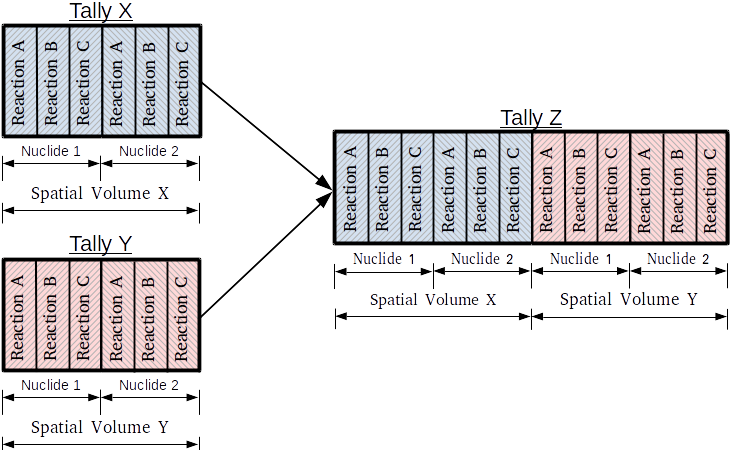
\includegraphics[width=0.6\linewidth]{figures/tally-merge}
  \caption{}
\end{subfigure}
\begin{subfigure}{\textwidth}
  \centering
  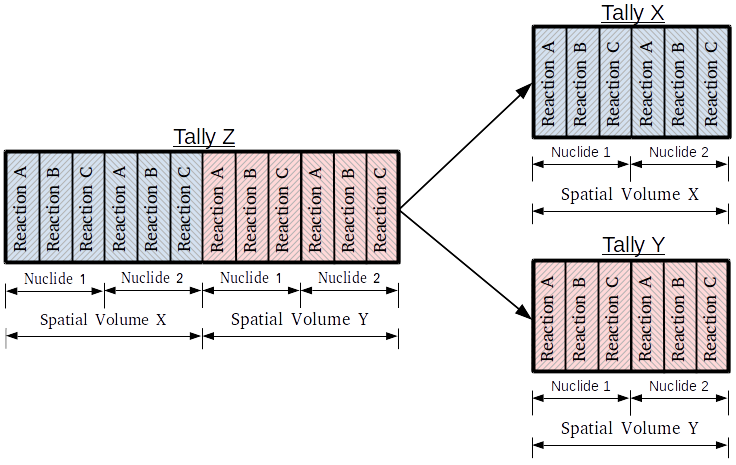
\includegraphics[width=0.6\linewidth]{figures/tally-slice}
  \caption{}
\end{subfigure}
\caption{Two \texttt{Tally} objects for different spatial volumes merged into a single \texttt{Tally} (a). A single \texttt{Tally} is sliced by spatial volume into two distinct \texttt{Tally} objects (b).}
\label{fig:tally-merge-slice}
\end{figure}

%%%%%%%%%%%%%%%%%%%%%%%%%%%%%%%%
\subsubsection{Tally Arithmetic}
\label{subsubsec:tally-arithmetic}

A variety of reaction rate and flux tallies must be arithmetically combined in order to compute MGXS with Monte Carlo. At the most general level, a reaction rate tally must be divided by a flux tally for each energy group, nuclide, and tally volume. The Python API provides a novel feature known as \emph{tally arithmetic} to enable the arithmetic combinations of tallies with efficient vectorized numerical operations across energy groups, nuclides, and spatial tally zones.

Tally arithmetic is an object-oriented data-processing feature that arithmetically combines two or more tallies and/or scalar values into new \emph{derived tallies}. The Python API overloads the \texttt{Tally} class' operators for addition, subtraction, multiplication, and division. Furthermore, the \texttt{Tally} class supports summation and averaging operations across some or all of its filter, nuclide, or score bins.

Multigroup cross sections may be simply and efficiently computed with tally arithmetic. For example, the code snippet in \cref{lst:python-input} illustrates how tally slicing and arithmetic are used to compute a total MGXS. The total MGXS that is returned from the tally division operation is encapsulated within a \texttt{Tally} object. This is the approach used by the MGXS generation module created for OpenMC.

\lstinputlisting[language=Python, basicstyle=\ttfamily\scriptsize, caption={MGXS calculation with tally arithmetic.}, label={lst:python-input}]{listings/tally-arithmetic.py}

Tally arithmetic automatically propagates the uncertainties of the tally operands through the arithmetic operation to estimate the uncertainty of the resulting derived tally. Estimates of the variance for derived tallies are deduced from standard error propagation theory~\cite{bevington2003data}. The division operator is used primarily to compute MGXS from MC tallies. Consider two random variables $X$ and $Y$, generated from distributions with variances $\sigma_{X}^2$ and $\sigma_{Y}^2$, that are divided into a new random variable $Z$ with variance $\sigma_{Z}^2$:

\begin{equation}
\label{eqn:div-prop}
\sigma_{Z}^{2} \approx Z^{2}\left[\left(\frac{\sigma_{X}}{X}\right)^{2} + \left(\frac{\sigma_{Y}}{Y}\right)^{2} - 2\frac{\sigma_{XY}}{Z}\right].
\end{equation}

\noindent The variables $X$ and $Y$ may correspond to reaction rates and the flux tallies, while $Z$ could correspond to the MGXS.

The covariance $\sigma_{XY}$ is not generally computable by using the standard formulation for a tally estimator in a Monte Carlo simulation. Although one could estimate the covariance using ensemble statistics, this approach is typically infeasible. Instead, the covariance term in \cref{eqn:div-prop} is currently neglected by OpenMC's implementation of tally arithmetic. In general, the random variables for reaction rates and fluxes in the same volume of phase space are highly correlated, such that a conservative estimate of the variance for MGXS is obtained by neglecting the covariance.

%%%%%%%%%%%%%%%%%%%%%%%%%%%%%%%%%%%%%
\subsection{Distributed Cell Tallies}
\label{subsec:distribcells}

%Many Monte Carlo codes, including OpenMC, use some variant of combinatorial geometry (CG) because it can represent arbitrary, repeating geometries such as fuel pins and assemblies. However, the CG approach is challenged by applications which require tallies in each instance of a repeated cell throughout a reactor geometry. The ``brute force'' solution is to instantiate a unique cell for each distinct tally zone. However, this defeats the purpose of using CG for its compact representation, and it is not scalable to problems with large tally datasets such as those considered in this thesis.

The \emph{distributed cell tally} algorithm was implemented in OpenMC \cite{lax2014distribcell} to permit simply defined spatial tally zones across repeated cell instances. The distributed cell tally algorithm, abbreviated as the \emph{distribcell} algorithm, may be used to compute spatially varying MGXS across fuel pin cell instances. The distribcell algorithm classifies each unique cell instance using a process that consumes orders of magnitude less memory than would be required by the ``brute force'' approach necessary to accomplish the same objective with other commonly used Monte Carlo codes. Only a single transparent line of XML input is necessary to define a distribcell tally that may span across an arbitrary number of instances for a particular cell. Furthermore, the Python API may be used to perform efficient vectorized transformations of distribcell tally data stored as contiguous NumPy arrays to compute MGXS.

%%%%%%%%%%%%%%%%%%%%%%%%%%%%%%%%%%%%%%%%%%%%%%%%%%%%%%%%%%%%%%%%%%%%%%%%%%%%%%%
\section{Design and Implementation}
\label{sec:design}
%%%%%%%%%%%%%%%%%%%%%%%%%%%%%%%%%%%%%%%%%%%%%%%%%%%%%%%%%%%%%%%%%%%%%%%%%%%%%%%

We have outlined in \cref{sec:mgxs-mc} procedures for estimating multi-group cross sections based on flux and reaction rate tallies from a Monte Carlo code. It is conceptually simple to have a Monte Carlo code compute these tallies and directly report a macroscopic or microscopic multi-group cross section as part of the output of the code. Indeed, this is the approach adopted by the Serpent Monte Carlo code\cite{leppanen2016homog}. The approach taken in OpenMC is fundamentally different---instead of having the solver directly calculate and report MGXS, the standard output of the code only includes flux and reaction rate values directly. After a simulation is complete, the reported tallies are read by a set of Python classes and the calculation of MGXS is performed as a post-processing task from within a Python Application Programming Interface (API). Before we outline the MGXS implementation within the Python API, we first discuss the OpenMC code and its Python API.

%%%%%%%%%%%%%%%%%%%%%%%%
\subsection{OpenMC Code}
\label{subsec:openmc-overview}

OpenMC is an open source Monte Carlo particle transport code which is primarily intended for use in neutron criticality calculations. It is capable of simulating three-dimensional models using constructive solid geometry. It also supports both continuous-energy and multi-group cross section data in a native HDF5\cite{koranne2011hdf5} data format\cite{romano2017epjwoc} that can be generated from ACE files.

OpenMC features a flexible, low-overhead tally system that enables users to obtain physical results of interest. Tallies are defined by combinations of \emph{filters} and \emph{scores}. Each filter limits what events can score to the tally based on the phase space variables. For example, a filter could limit scoring events to particles traveling within in a specified cell or a specified range of pre-collision energies. Each score identifies a physical quantity to be scored when an event occurs that matches the specified filters. Looking at \cref{eqn:inner-prod}, filters correspond to the limits of integration and scores correspond to the integrand itself:
\begin{equation}
\langle \Sigma_x, \psi \rangle = \underbrace{\int_{V} \int_{S} \int_{E}}_{\text{filters}} \underbrace{\Sigma_{x}(\mathbf{r},E)\psi(\mathbf{r},E,\mathbf{\Omega})}_{\text{scores}} \mathrm{d}E\mathrm{d}\mathbf{\Omega}\mathrm{d}\mathbf{r}
\end{equation}
In addition to filters and scores, it is also possible to obtain reaction rates by individual nuclides by specifying a list of nuclides. Each tally definition is permitted to have multiple filters, multiple scores, and multiple nuclides. Additionally, the estimator used to score events can also be specified on a per-tally basis.

A wide range of filters and scores have been implemented as of the version 0.9.0 release of OpenMC\cite{openmc-090}. The available filters can generally be categorized as follows:
\begin{itemize}
\item \emph{Spatial domain}: Tally events by universe, material, cell, mesh
\item \emph{Energy domain}: Tally events based on both incoming and outgoing particle energy
\item \emph{Angle domain}: Tally events based on a particle's polar and azimuthal direction or scattering angle
\item \emph{Energy function}: Multiplies tally scores by an arbitrary function of incident energy
\item \emph{Delayed group}: Tally events which produced neutrons in particular delayed groups
\end{itemize}
The available scores in version 0.9.0 include: particle flux, all invidual reaction rates, neutron production from fission (total, prompt, or delayed), Legendre and spherical harmonic scattering moments, spherical harmonic flux moments, inverse velocity, recoverable fission energy release, and the delayed neutron production-weighted decay rate. Taken together, these filters and scores permit all inner products identified in \cref{tab:tally-types} to be estimated via tallies in OpenMC.

%%%%%%%%%%%%%%%%%%%%%%%
\subsection{Python API}
\label{subsec:pyapi}

In addition to the main transport solver, a fully-featured Python API enables programmatic pre- and post-processing for OpenMC\cite{boyd2016bigdata}. The API enables tight coupling of input generation, simulation execution, and tally data analysis within dynamic Python scripts that form their own ``input files.'' In addition, the API makes it possible to leverage the extensive ecosystem of Python packages for scientific computing alongside OpenMC in a simulation workflow. The following sections describe the API and some of the core features which comprise the software stack developed to support the MGXS generation module created for OpenMC.

The Python API is a user-friendly, complementary (and optional) addition to the OpenMC codebase. OpenMC is written in Fortran 2008 and uses eXtensible Markup Language (XML) input files to describe the simulation materials, geometry, tallies, and settings. Although XML is often hailed as both human-readable and machine-readable, it can be cumbersome to write by hand for large and complicated reactor models. The Python API leverages Python's standard library to automatically generate XML input files used by the OpenMC executable. Instead of writing XML files by hand, Python scripts are used to describe one or more OpenMC simulations, including those used to generate MGXS with OpenMC.

The OpenMC Python API adheres to object-oriented software design principles with extensible class definitions. A user instantiates, manipulates, and connects objects representing items such as the materials, geometry, and tallies to construct an OpenMC simulation. This is a scalable alternative workflow to traditional ``decks'' of ``cards'' in which data characterizing a simulation is specified in opaque ASCII files (e.g., integer identifiers for geometric primitives such as surfaces, cells, and universes). The Python API provides classes and functions to expose all features provided by OpenMC's XML input specifications.

In addition to its functionality for input generation, the Python API also includes a rich framework for tally data processing. The API eliminates the time-intensive and error-prone process of writing code to parse results from output files. The API is able to reconstruct the hierarchy of interconnected Python objects used to represent the materials, geometry and tallies from OpenMC's HDF5 output files. OpenMC's dynamic object-oriented data processing model---fusing the geometry and materials configuration with tallied data---enables the rapid calculation, indexing, and storage of MGXS from tallies over specified spatial domains.

%%%%%%%%%%%%%%%%%%%%%%%%%%%%%%%%%
%\subsubsection{Pandas DataFrames}
%\label{subsubsec:chap4-pandas-df}

The Python API encapsulates numerical tally data using $N$-dimensional array objects from the NumPy third-party package\cite{walt2011numpy}. Although OpenMC's NumPy interface to tally data is more flexible than simply reporting the data in ASCII files, NumPy arrays are relatively opaque containers for managing large tally datasets. A single OpenMC \texttt{Tally} object used for MGXS generation may encompass many different energy groups, nuclides and reaction types, yet all of this data is tabulated in a single contiguous NumPy array. As a result, it is challenging to implement general algorithms to inspect, index, and manipulate tally data in NumPy arrays for specific groups, nuclides or reactions.

The Pandas third-party package\cite{mckinney2010pandas} was utilized in the Python API to enable transparent tally data processing for MGXS generation. In particular, the \texttt{Tally} class includes a feature to construct a Pandas \texttt{DataFrame} object from tally data. Pandas DataFrames are modeled after data structures in the \textsf{R} programming language used to store data tables in a more accessible format than contiguous arrays. They support mixed-type data (e.g., strings and numbers) and allow the use of string keys or labels to index each column or row. The Python API builds Pandas DataFrames by annotating tally data with the filters, nuclides, and scores associated with each tally bin.

%%%%%%%%%%%%%%%%%%%%%%%%%%%%%%%%
\subsubsection{Tally Slicing and Merging}
\label{subsubsec:tally-slice-merge}

Two useful and related features in the OpenMC Python API for MGXS generation are \emph{tally merging} and \emph{tally slicing} as depicted in \cref{fig:tally-merge-slice}. It is intuitively useful to systematically create individual \texttt{Tally} objects for each spatial domain and reaction type when generating the OpenMC inputs necessary to compute MGXS. However, this necessarily leads to a large number (10$^2$ -- 10$^3$) of distinct tally objects for large, complex geometries, which poses a computational bottleneck since the overhead to tally in OpenMC scales as $\mathcal{O}(N)$ for $N$ tallies\footnote{Note that $N$ refers to the number of tally definitions, each of which can contain multiple filters, nuclides, and scores.}. To compensate for this, the Python API's \texttt{Tally} class automatically merges user-specified tallies for input generation. Similarly, the API supports the slicing of tallies to simplify downstream data processing which may comprise energy-, nuclide-, and/or reaction-dependent transformations of the tally data.

\begin{figure}
\begin{subfigure}{\textwidth}
  \centering
  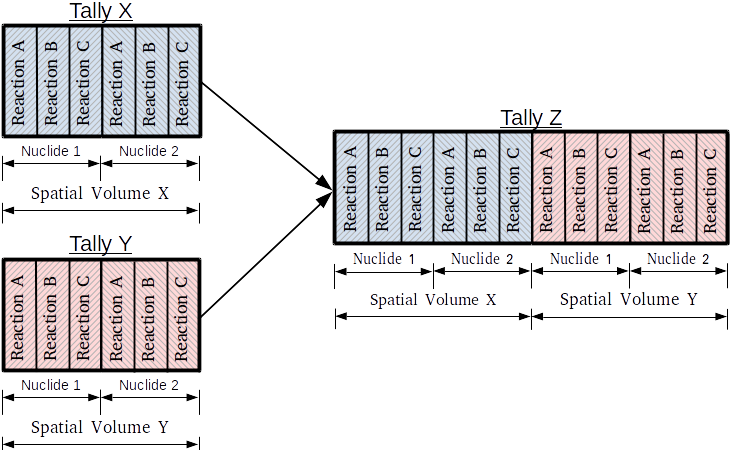
\includegraphics[width=0.6\linewidth]{figures/tally-merge}
  \caption{}
\end{subfigure}
\begin{subfigure}{\textwidth}
  \centering
  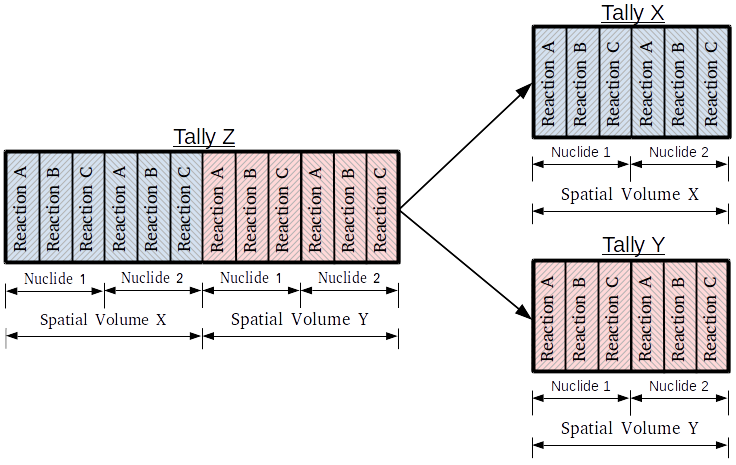
\includegraphics[width=0.6\linewidth]{figures/tally-slice}
  \caption{}
\end{subfigure}
\caption{Two \texttt{Tally} objects for different spatial volumes are merged into a single \texttt{Tally} (a). A single \texttt{Tally} is sliced by spatial volume into two distinct \texttt{Tally} objects (b).}
\label{fig:tally-merge-slice}
\end{figure}

%%%%%%%%%%%%%%%%%%%%%%%%%%%%%%%%
\subsubsection{Tally Arithmetic}
\label{subsubsec:tally-arithmetic}

A variety of reaction rate and flux tallies must be arithmetically combined in order to compute MGXS with Monte Carlo. At the most general level, a reaction rate tally must be divided by a flux tally for each energy group, nuclide and tally volume. The Python API provides a novel feature known as \emph{tally arithmetic} to enable arithmetic combinations of tallies with efficient vectorized numerical operations across energy groups, nuclides and spatial tally zones.

Tally arithmetic is an object-oriented data processing feature which arithmetically combines two or more tallies and/or scalar values into new \emph{derived tallies}. The tally arithmetic implementation in OpenMC overloads the operators for addition, subtraction, multiplication, division, and exponentiation in the Python API's \texttt{Tally} class. In addition, the \texttt{Tally} class supports summation or averaging operations across some or all of its filter, nuclide or score bins. The derived tallies produced from tally arithmetic provide the same rich functionality available for the \texttt{Tally} operands used in the arithmetic operation (e.g., Pandas DataFrames, tally arithmetic).

Multi-group cross sections may be simply and efficiently computed with tally arithmetic. For example, the following code snippet illustrates how tally slicing and arithmetic are used to compute a total MGXS. The total MGXS that is returned from the tally division operation is encapsulated within a \texttt{Tally} class. This is the approach used by the MGXS generation module created for OpenMC.

\lstinputlisting[language=Python, basicstyle=\ttfamily\scriptsize, caption={MGXS calculation with tally arithmetic.}, label={lst:python-input}]{listings/tally-arithmetic.py}

A primary objective of tally arithmetic is to rapidly transform tally data with automated uncertainty propagation. Estimates of the variance for derived tallies from tally arithmetic are deduced from standard error propagation theory~\cite{bevington2003data}. The division arithmetic operator is primarily used to to compute MGXS from MC tallies. Consider two random variables $X$ and $Y$, generated from distributions with variances $\sigma_{X}^2$ and $\sigma_{Y}^2$ which are divided into a new random variable $Z$ with variance $\sigma_{Z}^2$:

\begin{equation}
\label{eqn:div-prop}
\sigma_{Z}^{2} \approx Z^{2}\left[\left(\frac{\sigma_{X}}{X}\right)^{2} + \left(\frac{\sigma_{Y}}{Y}\right)^{2} - 2\frac{\sigma_{XY}}{Z}\right]
\end{equation}

\noindent The variables $X$ and $Y$ may correspond to tallies for reaction rates and the flux, respectively, while $Z$ could correspond to a MGXS.

The covariance $\sigma_{XY}$ is not generally computable using the standard formulation for a tally estimator in a Monte Carlo simulation. Although it would be possible to estimate the covariance using ensemble statistics, this is not often feasible. Instead, the covariance term in \cref{eqn:div-prop} is neglected by the current implementation of tally arithmetic. In general, the random variables for reaction rates and fluxes in the same volume of phase space are highly correlated, such that a conservative estimate of the variance for MGXS is obtained by neglecting the covariance.

%%%%%%%%%%%%%%%%%%%%%%%%%%%%%%%%%%%%%
\subsubsection{Distributed Cell Tallies}
\label{subsec:distribcells}

%Many Monte Carlo codes, including OpenMC, use some variant of combinatorial geometry (CG) because it can represent arbitrary, repeating geometries such as fuel pins and assemblies. However, the CG approach is challenged by applications which require tallies in each instance of a repeated cell throughout a reactor geometry. The ``brute force'' solution is to instantiate a unique cell for each distinct tally zone. However, this defeats the purpose of using CG for its compact representation, and it is not scalable to problems with large tally datasets such as those considered in this thesis.

The \emph{distributed cell tally} algorithm was implemented in OpenMC \cite{lax2014distribcell} to permit simply defined spatial tally zones across repeated cell instances. The distributed cell algorithm -- abbreviated as the \emph{distribcell} algorithm -- classifies each unique cell instance using a process which consumes orders of magnitude less memory than would be required by the ``brute force'' approach. Only a single transparent line of XML input is necessary to define a distribcell tally which may span across an arbitrary number of instances for a particular cell. Furthermore, the Python API may be used to perform efficient vectorized transformations of distribcell tally data stored as contiguous NumPy arrays. In particular, the distribcell tally algorithm may be used to compute spatially-varying MGXS across fuel pin cell instances.

%%%%%%%%%%%%%%%%%%%%%%%%%%%%%
\subsubsection{Multi-Group Mode}
\label{subsec:openmc-mg-mode}

\begin{itemize}[noitemsep]
\item support stochastic multi-group calculations
\item multiple scattering representations (Legendre moments, discrete bins)
\item use OpenMC to generate MGXS, then insert into identical model for MG calculation
\item mention angular-dependent MGXS, or save for later paper?
\end{itemize}

%%%%%%%%%%%%%%%%%%%%%%%%%%%%%%%%%%%%%%%%%%%%%%%%%%%%%%%%%%%%%%%%%%%%%%%%%%%%%%%
\subsection{Multi-Group Cross Section Module Design}
\label{sec:software}
%%%%%%%%%%%%%%%%%%%%%%%%%%%%%%%%%%%%%%%%%%%%%%%%%%%%%%%%%%%%%%%%%%%%%%%%%%%%%%%

The Python API features a module called \texttt{openmc.mgxs} that was designed to generate multi-group cross sections. The \texttt{openmc.mgxs} module is built atop the underlying core features in the rest of the API to support a seamless interface for both input generation and downstream data processing of MGXS from Python. In particular, one may specify the MGXS to compute and the \texttt{openmc.mgxs} module will construct the necessary \texttt{Tally} objects. The \texttt{Tally} objects may be easily exported to XML input files and used to containerize and process the tally data produced by an OpenMC simulation. The \texttt{openmc.mgxs} module thereby leverages the existing classes and features (e.g., tally arithmetic and Pandas DataFrames) provided by the Python API.

The \texttt{openmc.mgxs} module uses an object-oriented design based on an abstract \texttt{MGXS} class with subclasses for different cross section types. The \texttt{MGXS} subclasses, as listed in \cref{tab:mgxs-types}, compute macroscopic or microscopic multi-group constants in one or more arbitrary energy group structures from MC tallies. The \texttt{openmc.mgxs} module also includes a \texttt{Library} class which automates the construction of \texttt{MGXS} objects for different group structures, spatial domains, and reaction types.

\begin{table}[h!]
  \centering
  \caption{The multi-group cross section types implemented by the \texttt{openmc.mgxs} module.}
  \small
  \label{tab:mgxs-types}
  \vspace{6pt}
  \begin{tabular}{l l}
  \toprule
  \textbf{Class} &
  \textbf{Description} \\
  \midrule
  \multicolumn{2}{c}{\bf Prompt Neutron Constants} \\
  \midrule
  \texttt{AbsorptionXS} & Absorption \\
  \texttt{CaptureXS} & Radiative capture \\
  \texttt{Chi} & Fission emission spectrum \\
  \texttt{FissionXS} & Fission \\
  \texttt{InverseVelocity} & Inverse neutron velocity \\
  \texttt{KappaFissionXS} & Fission energy release \\
  \texttt{MultiplicityMatrixXS} & Scattering multiplicity matrix \\
  \texttt{NuFissionMatrixXS} & Fission production matrix \\
  \texttt{ScatterXS} & Scattering \\
  \texttt{ScatterMatrixXS} & Scattering matrix \\
  \texttt{ScatterProbabilityMatrixXS} & Scattering probability matrix \\
  \texttt{TotalXS} & Total collision \\
  \texttt{TransportXS} & Transport-corrected total collision \\
  \midrule
  \multicolumn{2}{c}{\bf Delayed Neutron Constants} \\
  \midrule
  \texttt{Beta} & Delayed neutron fraction \\
  \texttt{ChiDelayed} & Delayed fission spectrum \\
  \texttt{DecayRate} & Delayed neutron precursors decay rate \\
  \texttt{DelayedNuFissionXS} & Fission delayed neutron production \\
  \texttt{DelayedNuFissionMatrixXS} & Fission delayed neutron production matrix \\
  \bottomrule
\end{tabular}
\end{table}


%%%%%%%%%%%%%%%%%%%%%%%%%%%%%
\subsubsection{XML Input Generation}
\label{subsec:xml-inputs}

\begin{itemize}[noitemsep]
\item workflow: create Python model, create \texttt{Library}, export to XML
\item code snippet?
\end{itemize}

%%%%%%%%%%%%%%%%%%%%%%%%%%%%%
\subsubsection{Data Processing}
\label{subsec:data-processing}

\begin{itemize}[noitemsep]
\item refer to PyAPI features that are ``inherited'' by \texttt{openmc.mgxs}:
  \begin{itemize}[noitemsep]
  \item Pandas DataFrames, tally arithmetic/slicing/merging, ...
  \end{itemize}
\end{itemize}

%%%%%%%%%%%%%%%%%%%%%%%%%
\subsubsection{Data Storage}
\label{subsec:data-storage}

The \texttt{openmc.mgxs} module was developed with general design principles to generate MGXS for any multi-group neutron transport code. Although the module does not explicitly support any multi-group codes, it can export MGXS data to a variety of data storage formats, including Comma-Separated Values (CSV) and HDF5. The exported MGXS files may be easily transformed into the database or input files required by a particular multi-group code.

%%%%%%%%%%%%%%%%%%%%%%%%%%%%%%%%%%%%%%%%%%%%%%%%%%%%%%%%%%%%%%%%%%%%%%%%%%%%%%%
\subsection{Features}
\label{sec:features}
%%%%%%%%%%%%%%%%%%%%%%%%%%%%%%%%%%%%%%%%%%%%%%%%%%%%%%%%%%%%%%%%%%%%%%%%%%%%%%%


%%%%%%%%%%%%%%%%%%%%%%%%%%%%%%%%%%%%%%%%%%%%
\subsubsection{Energy Condensation}
\label{subsec:energy-condense}

The module supports energy condensation in downstream data processing which is useful for exploring approximation bias in various energy group structures. For example, MGXS may be computed in some ``fine'' energy group structure and the tally data subsequently condensed to some coarser group structure \texttt{coarse_groups} for multi-group calculations with the \texttt{MGXS.get_condensed_xs(coarse_groups)} Python class method. Energy condensation may be performed to arbitrarily defined coarse group structures provided the coarse group boundaries coincide with boundaries in the fine group structure.


%%%%%%%%%%%%%%%%%%%%%%%%%%%%%%%%%%%%%%%%%%%%
\subsubsection{Pin-Wise Spatial Homogenization}
\label{subsec:pinwise-homogenize}

The \texttt{openmc.mgxs} module is designed to perform spatial homogenization on heterogeneous tally meshes for fine-mesh transport codes. In OpenMC parlance, MGXS may be computed for material, cell or universe spatial domains. In addition, the module supports MGXS calculations for repeated cell instances using distribcell spatial tally domains\cite{lax2014distribcell}. Spatial homogenization across some subset of distributed cell instances \texttt{cell_instances} can be performed using the \texttt{MGXS.get_subdomain_avg_xs(cell_instances)} Python class method.

%The \texttt{openmc.mgxs} module may also perform spatial homogenization on structured Cartesian tally meshes for coarse mesh multi-group calculations..


%%%%%%%%%%%%%%%%%%%%%%%%%%%%%%%%%%%%%%%%%%%%
\subsubsection{Microscopic MGXS}
\label{subsec:micro-macro}

I hear it is unique that we can calculate micros?


%%%%%%%%%%%%%%%%%%%%%%%%%%%%%%%%%%%%%%%%
\subsubsection{Isotropic in Lab Scattering}
\label{subsec:iso-in-lab}

A unique option for isotropic in lab scattering is implemented in the OpenMC code. The isotropic in lab feature, abbreviated as \emph{iso-in-lab}, may be useful to quantify the ability of multi-group codes to capture anisotropic scattering effects with higher order scattering matrices or transport correction schemes. The iso-in-lab feature is implemented as an optional attribute for each nuclide or element in a simulation. When iso-in-lab scattering is specified for a nuclide or element, the outgoing neutron energy is sampled from the scattering laws prescribed by the continuous energy cross section library, but the outgoing neutron direction of motion is sampled from an isotropic in lab distribution.

%%%%%%%%%%%%%%%%%%%%%%%%%%%%%
\subsection{Tally Estimators}
\label{subsec:tally-est}

\begin{itemize}[noitemsep]
\item Table of the tally estimators acceptable for each MGXS type
\item Mention tally estimators can be toggled? Or discuss in software design?
\item Add footnote mentioning consistent scattering formulation
\end{itemize}

\begin{table}[h!]
  \centering
  \caption{The tally estimators supported by each MGXS type.}
  \small
  \label{tab:mgxs-tally-estimators}
  \vspace{6pt}
  \begin{tabular}{l c c c}
  \toprule
  \textbf{Class} &
  \textbf{Analog} &
  \textbf{Collision} &
  \textbf{Track-length} \\
  \midrule
  \multicolumn{4}{c}{\bf Prompt Neutron Constants} \\
  \midrule
  \texttt{AbsorptionXS} & \cmark & \cmark & \cmark \\
  \texttt{CaptureXS} & \cmark & \cmark & \cmark \\
  \texttt{Chi} & \cmark & \xmark & \xmark \\
  \texttt{FissionXS} & \cmark & \cmark & \cmark \\
  \texttt{InverseVelocity} & \cmark & \cmark & \cmark \\
  \texttt{KappaFissionXS} & \cmark & \cmark & \cmark \\
  \texttt{MultiplicityMatrixXS} & \cmark & \xmark & \xmark \\
  \texttt{NuFissionMatrixXS} & \cmark & \xmark & \xmark \\
  \texttt{ScatterXS} & \cmark & \cmark & \cmark \\
  \texttt{ScatterMatrixXS} & \cmark & \xmark & \xmark \\
  \texttt{ScatterProbabilityMatrixXS} & \cmark & \xmark & \xmark \\
  \texttt{TotalXS} & \cmark & \cmark & \cmark \\
  \texttt{TransportXS} & \cmark & \xmark & \xmark \\
  \midrule
  \multicolumn{4}{c}{\bf Delayed Neutron Constants} \\
  \midrule
  \texttt{Beta} & \cmark & \cmark & \cmark \\
  \texttt{ChiDelayed} & \cmark & \xmark & \xmark \\
  \texttt{DecayRate} & \cmark & \cmark & \cmark \\
  \texttt{DelayedNuFissionXS} & \cmark & \cmark & \cmark \\
  \texttt{DelayedNuFissionMatrixXS} & \cmark & \xmark & \xmark \\
  \bottomrule
\end{tabular}
\end{table}

%%%%%%%%%%%%%%%%%%%%%%%%%%%%%%%%%%%%%%%%%%%%%%%%%%%%%%%%%%%%%%%%%%%%%%%%%%%%%%%
\section{Validating the OpenMC MGXS Generation Module}
\label{sec:validate}
%%%%%%%%%%%%%%%%%%%%%%%%%%%%%%%%%%%%%%%%%%%%%%%%%%%%%%%%%%%%%%%%%%%%%%%%%%%%%%%

This section provides a case study to validate the \texttt{openmc.mgxs} module. \cref{subsec:benchmarks} introduces two Pressurized Water Reactor (PWR) benchmarks and the reference results computed with OpenMC. MGXS were generated with \texttt{openmc.mgxs} for both benchmarks as discussed in \cref{subsec:openmc} and then used for multi-group calculations with the OpenMOC code highlighted in \cref{subsec:openmoc}. The continuous energy and multi-group solutions are compared in \cref{subsec:results}.


%%%%%%%%%%%%%%%%%%%%%%%%%%%%%%%%%%%%%%%%%%%%%
\subsection{Benchmarks and Reference Results}
\label{subsec:benchmarks}

Two benchmarks were derived from the Benchmark for Evaluation And Validation of Reactor Simulations (BEAVRS) PWR model~\cite{horelik2013beavrs} to validate the \texttt{openmc.mgxs} module. Both benchmarks included a heterogeneous composition of 1.6\% and 3.1\% enriched UO$_2$ fuel, borated water, zircaloy, helium, air, borosilicate glass and stainless steel. The isotopic compositions of the materials and the geometric configurations of each pin type were identical to those given in the BEAVRS specifications and are not reproduced here. The continuous energy cross sections were from the ENDF/B-VII.1 library~\cite{mcnpx2003manual} evaluated at 600K for hot power conditions.

The two benchmarks are illustrated in \cref{fig:benchmarks-materials}. The first benchmark was a fuel assembly comprised of 264 pins of 1.6\% enriched fuel, 24 control rod guide tubes (CRGTs) and a single central instrument tube. The assembly was modeled with reflective boundary conditions. The second benchmark was a 2$\times$2 colorset of fuel assemblies surrounded by a water reflector on the bottom and right. The top-left and bottom-right fuel assemblies were identical to the single assembly benchmark. The top-right and bottom-left assemblies were comprised of 264 pins of 3.1\% enriched fuel, 20 CRGTs, four burnable poisons (BPs) and a central instrument tube. The colorset was modeled with reflective boundaries on the top and left and vacuum boundaries on the bottom and right. Although BEAVRS is an axially heterogeneous 3D core model, both benchmarks were fabricated in 2D due to the geometric constraints in OpenMOC.

\begin{figure}[h!]
\centering
\begin{subfigure}{0.45\textwidth}
  \centering
  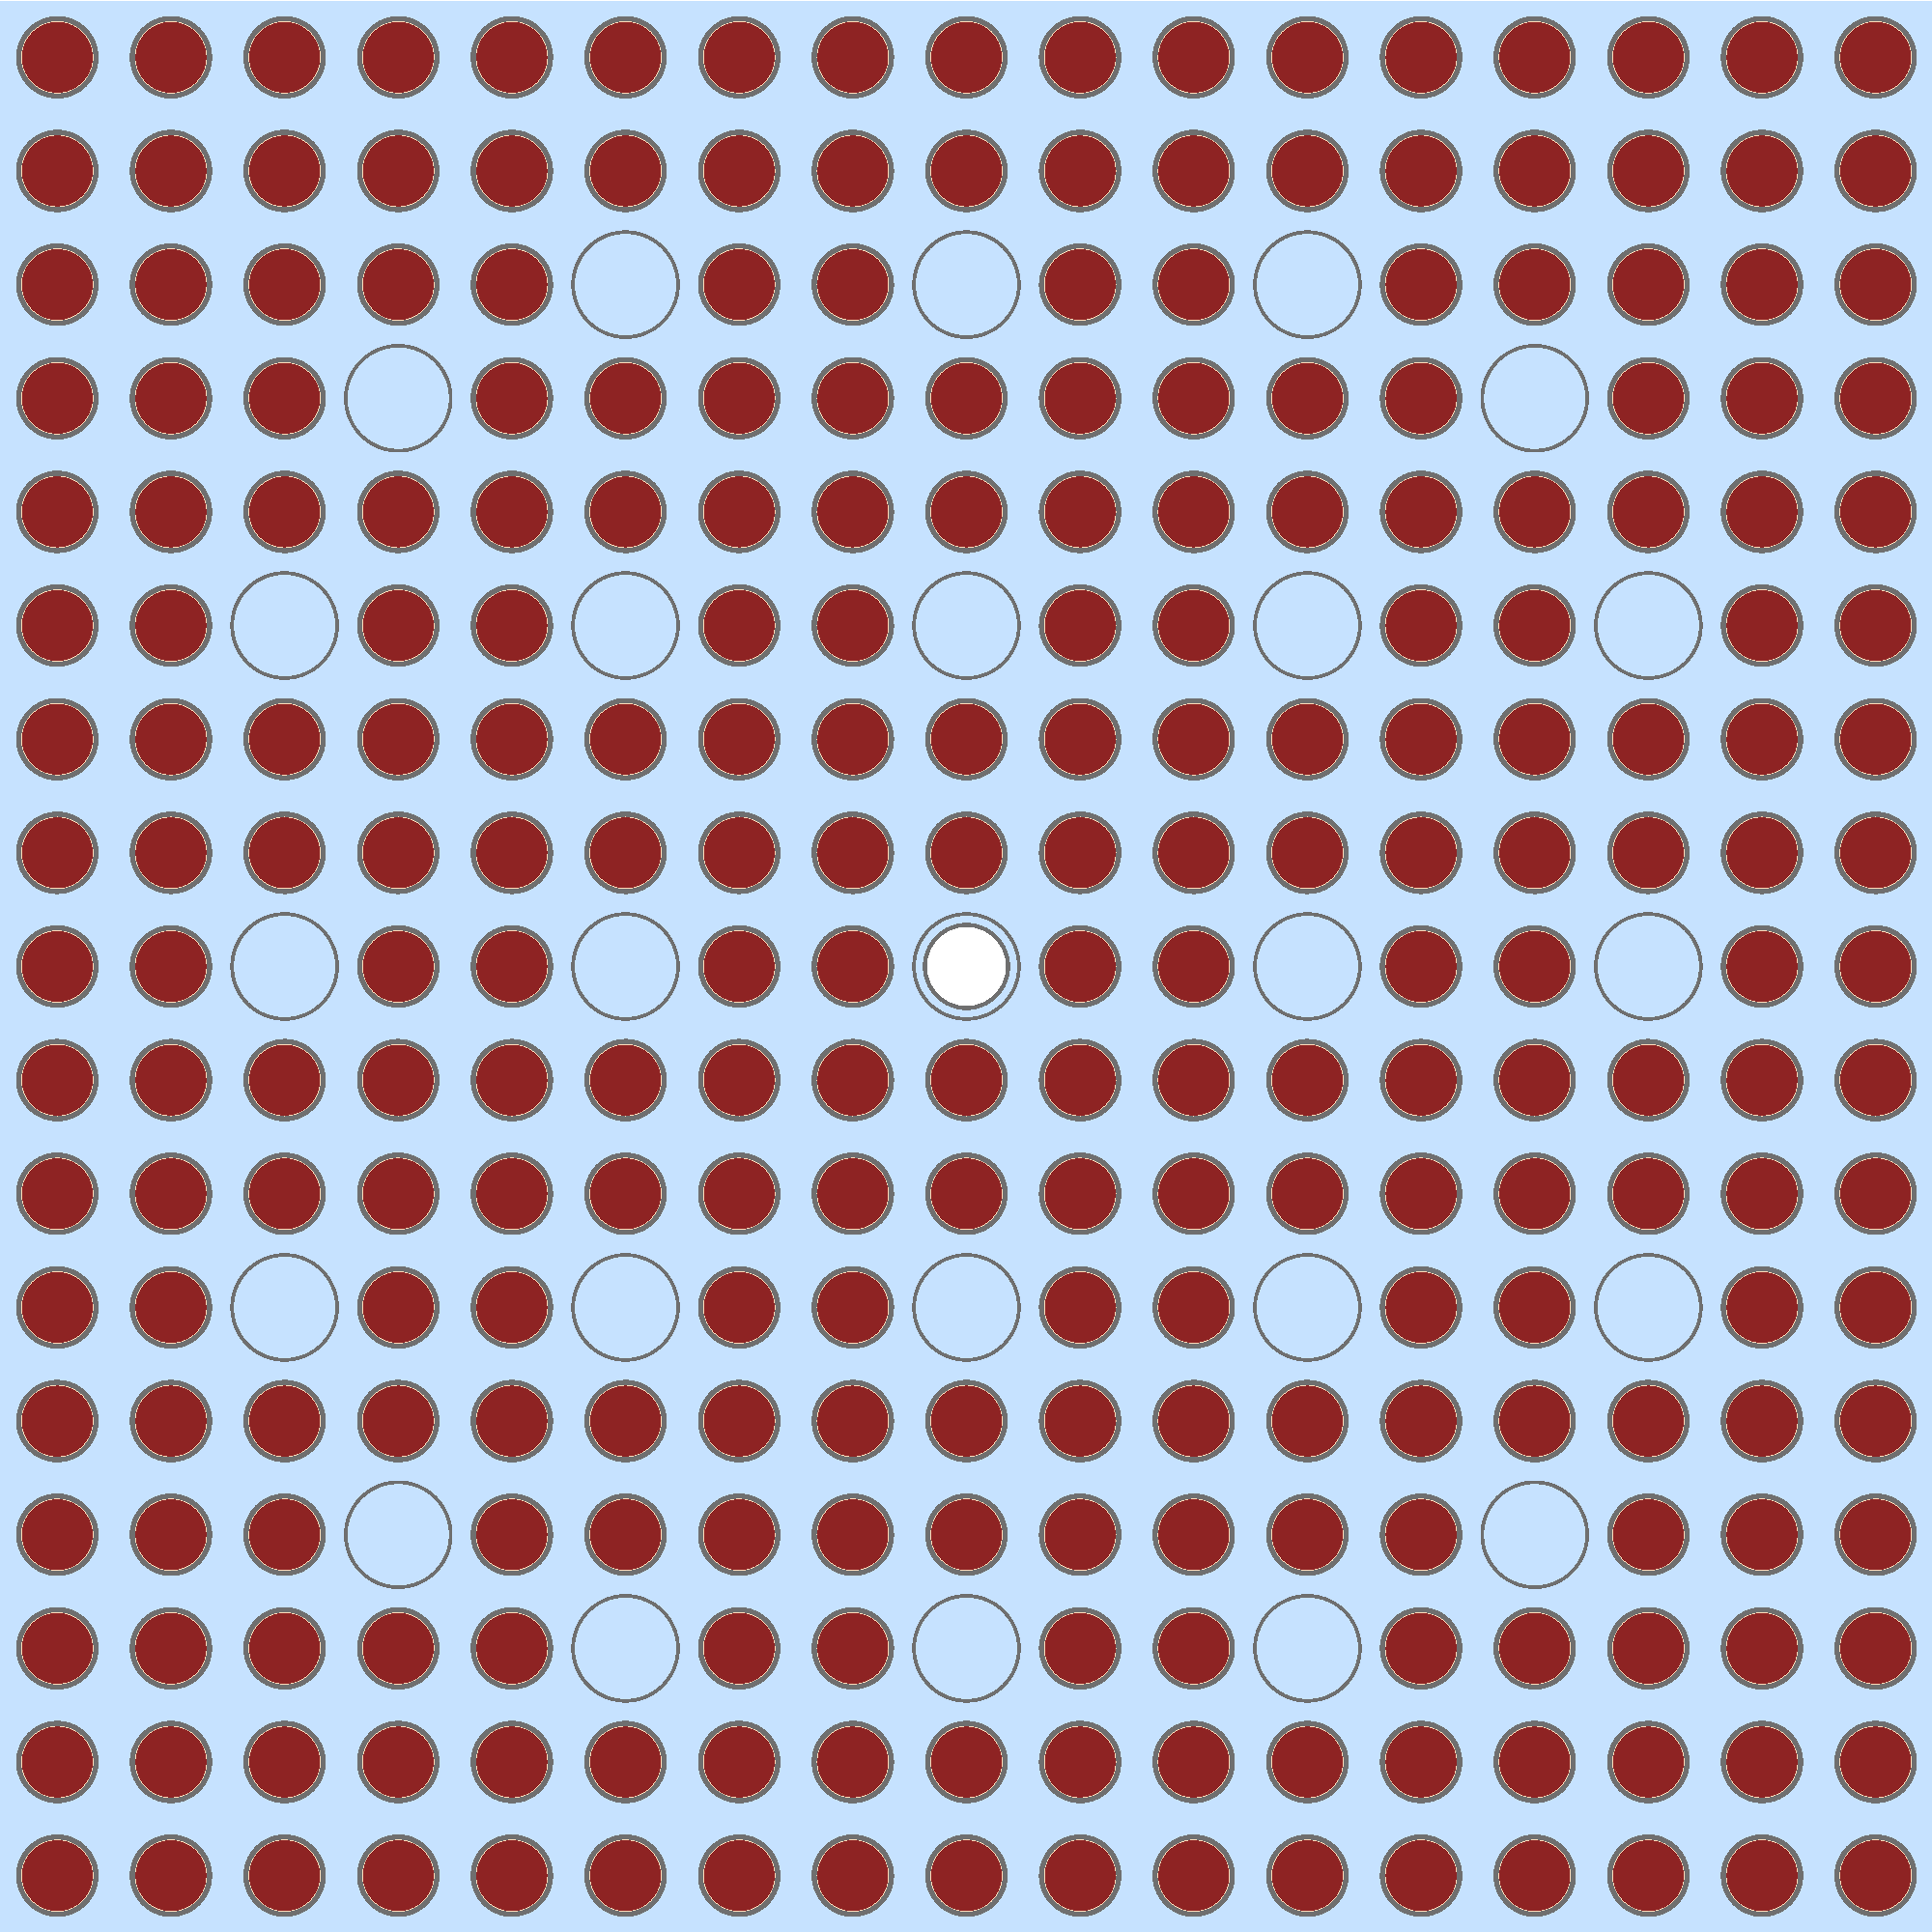
\includegraphics[width=0.8\linewidth]{figures/assembly/geometry}
  \caption{}
  \label{fig:benchmarks}
\end{subfigure}
\begin{subfigure}{0.45\textwidth}
  \centering
  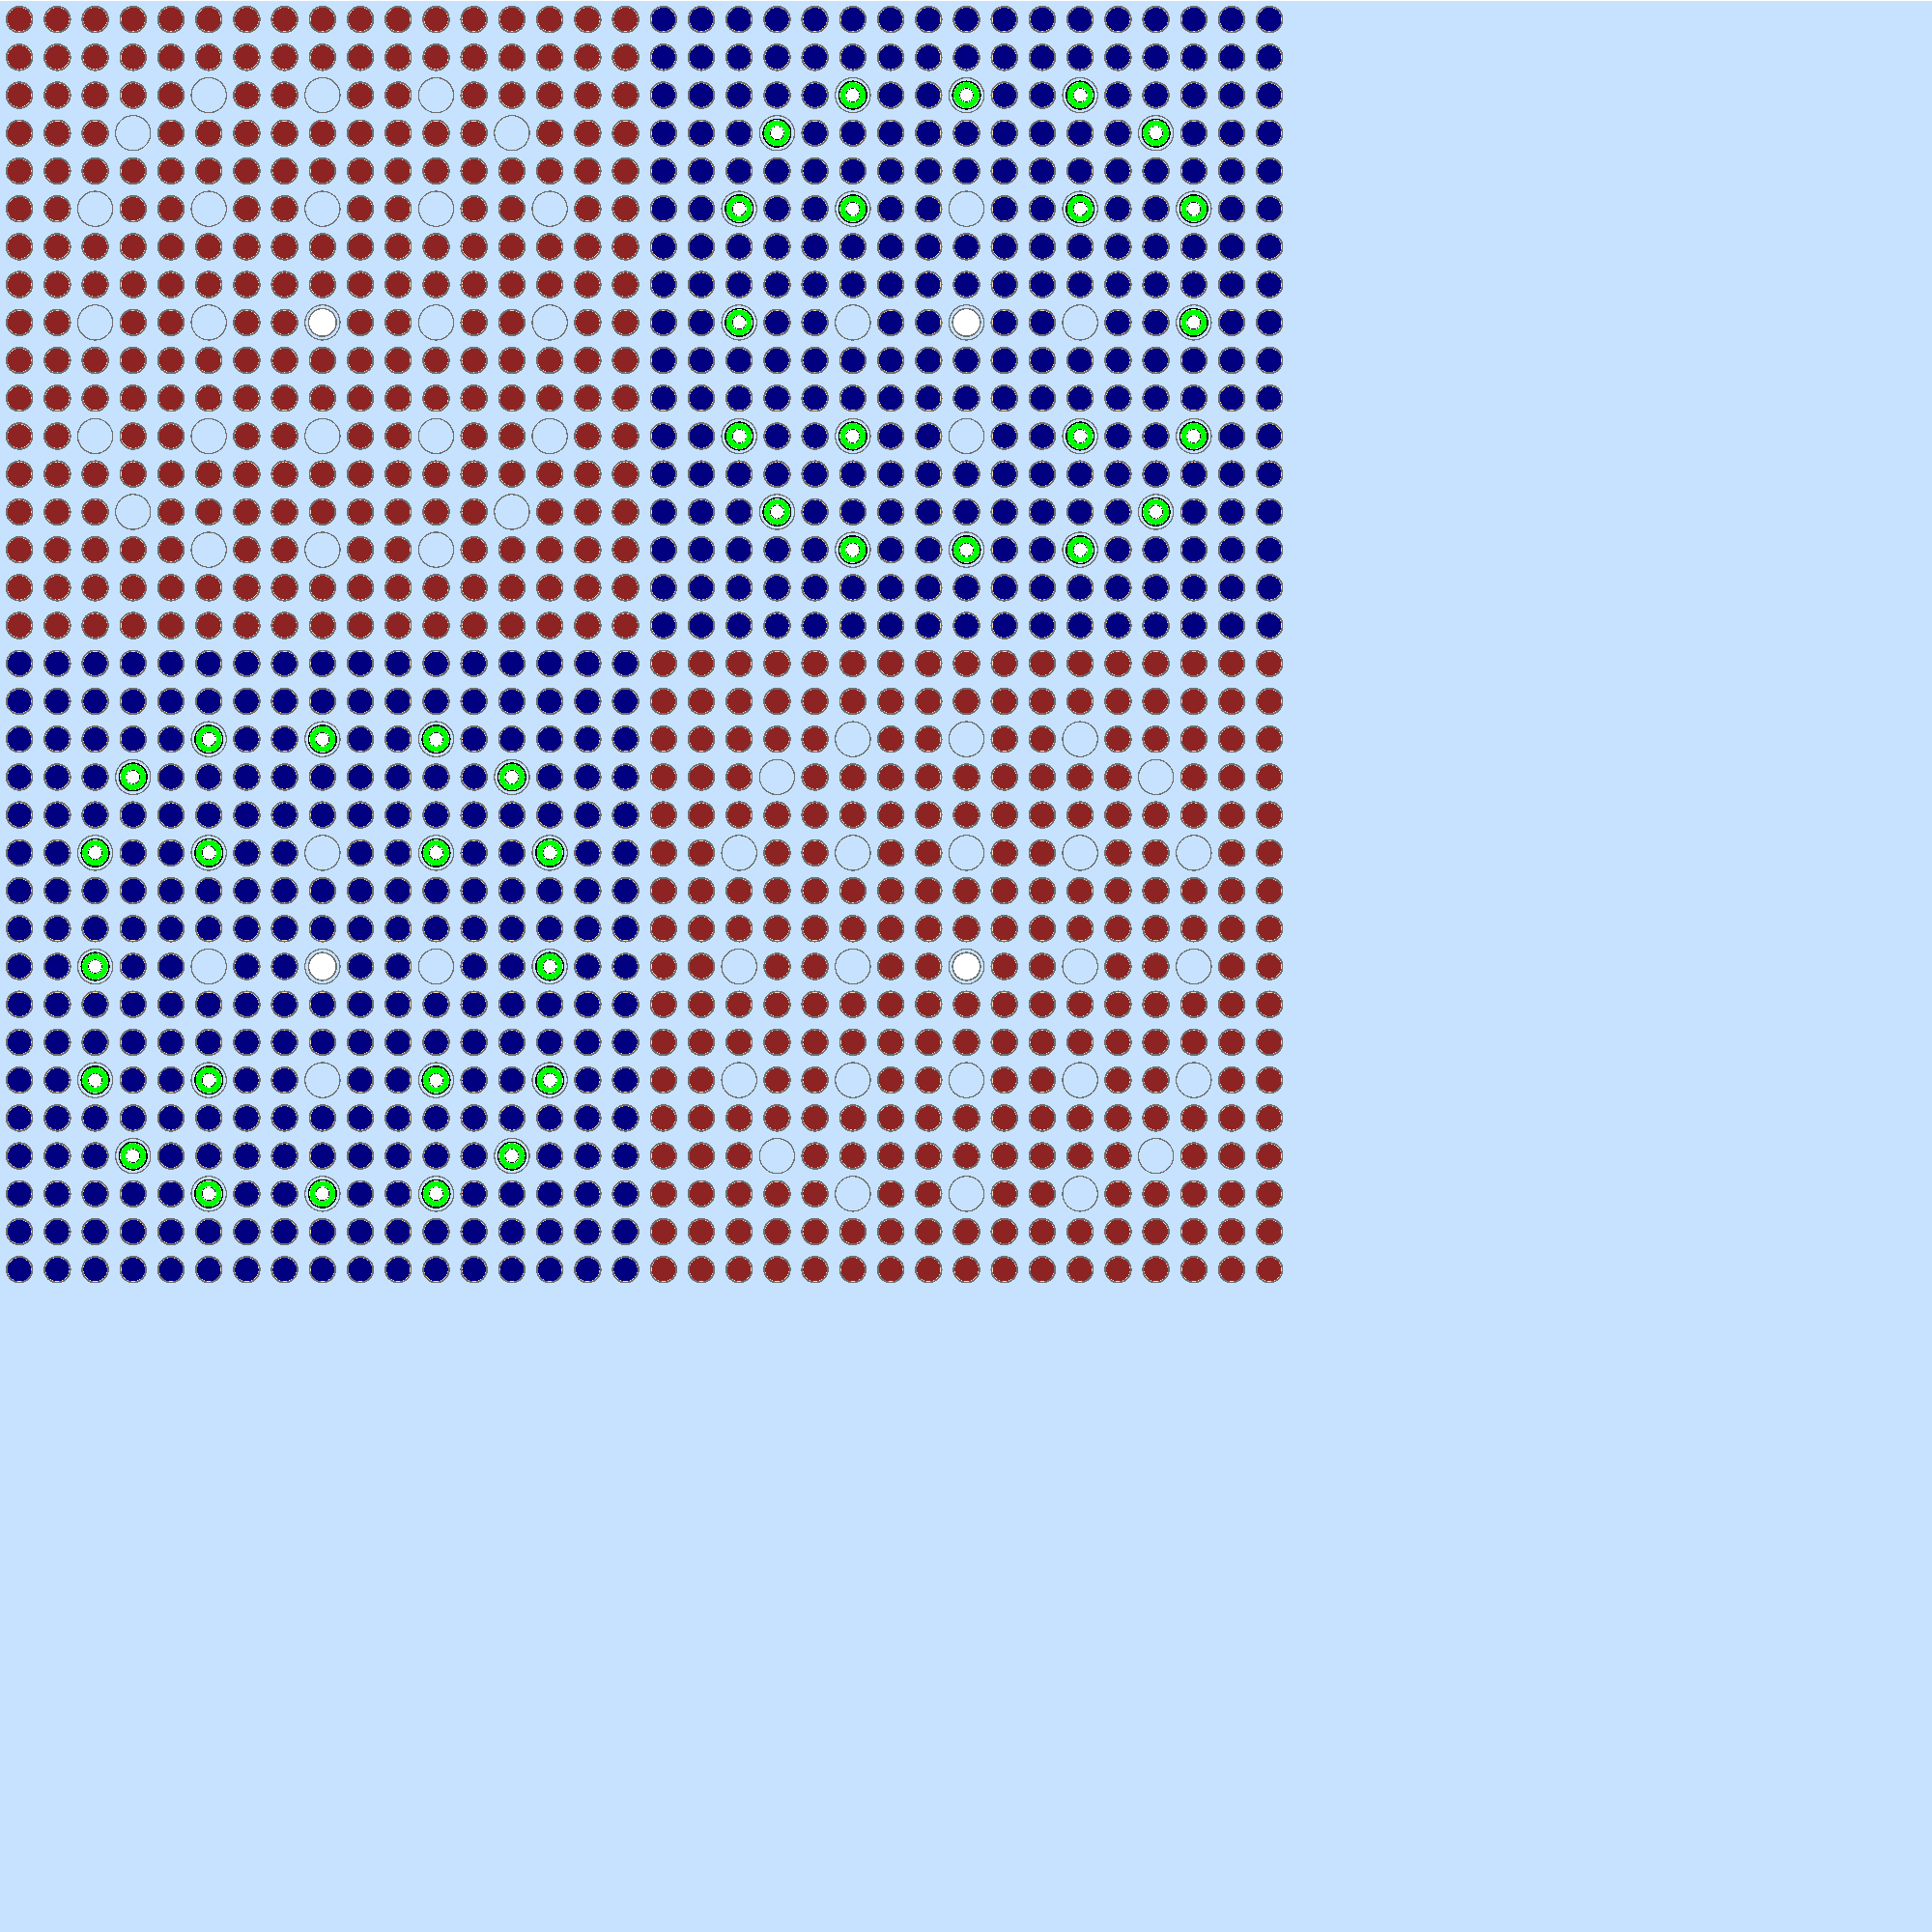
\includegraphics[width=0.8\linewidth]{figures/colorset/geometry}
  \caption{}
  \label{fig:benchmarks-colorset}
\end{subfigure}
\caption{The assembly (a) and colorset (b) benchmark geometries.}
\label{fig:benchmarks-materials}
\end{figure}

OpenMC simulations were used to compute both the MGXS as well as reference eigenvalues and pin-wise fission rates for both benchmarks. The reference solutions were computed with 100 inactive and 900 active batches of 10$^7$ particles histories per batch. The OpenMC reference eigenvalues and their associated 1-sigma uncertainties are reported in \cref{tab:keff-reference}. Rectilinear, pin-wise tally meshes were used to compute the reference energy-integrated fission rate spatial distributions shown in \cref{fig:benchmarks-fiss-rates}. The fission rates were normalized to the mean of the non-zero fission rates. The rates in the CRGTs, BPs, and instrument tubes are all zero and are shaded in white. The fission rates have 1-sigma uncertainties of less than 0.08\%.

\begin{table}[h!]
  \centering
  \caption{Reference OpenMC eigenvalues for each benchmark.}
  \label{tab:keff-reference}
  \begin{tabular}{c c}
  \toprule
  {\bf Assembly} &
  {\bf Colorset} \\
  \midrule
  0.99326 $\pm$ 0.00001 & 0.94574 $\pm$ 0.00001 \\
  \bottomrule
\end{tabular}
\end{table}

\begin{figure*}[h!]
\centering
\begin{subfigure}{0.45\textwidth}
  \centering
  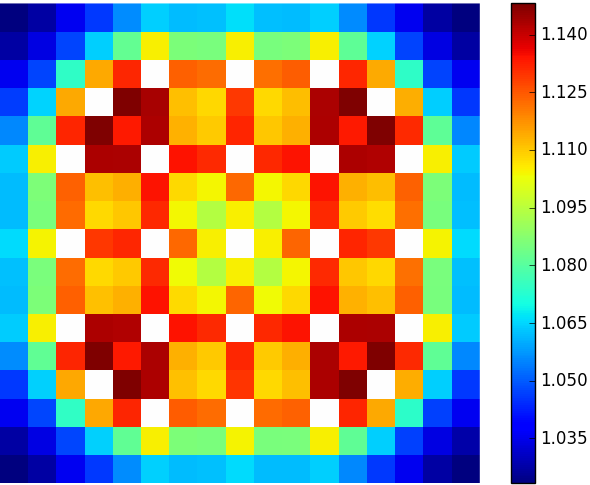
\includegraphics[width=0.8\linewidth]{figures/assembly/fission-rates}
  \caption{}
  \label{fig:fiss-assm}
\end{subfigure}%
\begin{subfigure}{0.45\textwidth}
  \centering
  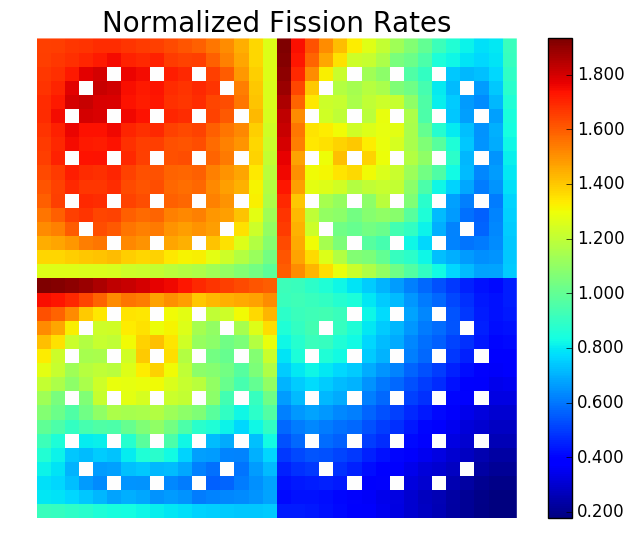
\includegraphics[width=0.8\linewidth]{figures/colorset/fission-rates}
  \caption{}
  \label{fig:capt-assm}
\end{subfigure}
\caption{Normalized reference OpenMC fission rates for the assembly (a) and colorset (b) benchmarks.}
\label{fig:benchmarks-fiss-rates}
\end{figure*}


%%%%%%%%%%%%%%%%%%%%%%%%%%%%%%%%%%%%%%%%%%%%%%%%%%%%%%%%%%%%
\subsection{MGXS Generation with OpenMC}
\label{subsec:openmc}

The \texttt{openmc.mgxs} module was employed to generate MGXS tallied in CASMO's seventy energy group structure \cite{rhodes2006casmo}. Two OpenMC eigenvalue calculations were performed for the 1.6\% and 3.1\% enriched fuel pins, each in an infinite, repeating array\footnote{An infinite, repeating array of fuel pins is modeled by a single fuel pin with reflective boundary conditions.}, to generate MGXS for the fuel, zircaloy cladding, helium gap and borated water moderator. An additional OpenMC eigenvalue calculation of the entire geometry for each benchmark was performed to generate MGXS for those pins lacking fissile materials (CRGTs, BPs and instrument tubes). The 70-group MGXS were subsequently condensed to CASMO's 8- and 2-group structures using the \texttt{openmc.mgxs} module's data processing features.

Each OpenMC simulation included 100 inactive and 900 active batches of 10$^{6}$ particle histories per batch. The OpenMC simulations used the ``iso-in-lab'' feature to eliminate scattering source anisotropy as one possible cause of approximation error between OpenMC and OpenMOC, since OpenMOC uses an isotropic scattering source.


%%%%%%%%%%%%%%%%%%%%%%%%%%%%%%%%%%%%%%%%%%%%%%%%%%%%%%%%%%%%
\subsection{Multi-Group Calculations with OpenMOC}
\label{subsec:openmoc}

The MGXS generated by OpenMC were supplied to OpenMOC \cite{boyd2014openmoc} for deterministic multi-group transport calculations. The OpenMOC code solves the method of characteristics form of the neutron transport equation for 2D fixed source and eigenvalue calculations. OpenMOC approximates the scattering source as isotropic and the neutron source as constant across each spatial zone. The OpenMOC simulations used a characteristic track laydown with 128 azimuthal angles and 0.05 cm spacing. The root mean square of the energy-integrated fission source in each spatial zone was converged to 10$^{-5}$. The eigenvalues and pin-wise fission rates computed by OpenMOC are compared to the OpenMC reference solutions for both benchmarks in the following section.


%%%%%%%%%%%%%%%%%%%%%%%%%%%%%%%%%%%%%%%%%%%%%%%%%%%%%%%%%%%%%%%%%%%%%%%%%%%%%%%
\subsection{Results}
\label{subsec:results}
%%%%%%%%%%%%%%%%%%%%%%%%%%%%%%%%%%%%%%%%%%%%%%%%%%%%%%%%%%%%%%%%%%%%%%%%%%%%%%%

The OpenMOC eigenvalues were compared to the reference OpenMC eigenvalues from \cref{tab:keff-reference}. The eigenvalue bias $\Delta k$ was calculated by comparing the eigenvalue $k_{eff}^{MOC}$ from OpenMOC to the reference eigenvalue $k_{eff}^{MC}$ computed by OpenMC in units of per cent mille (pcm):

\begin{equation}
\label{eqn:delta-rho}
\Delta k = \left(k_{eff}^{MOC} - k_{eff}^{MC}\right) \times 10^{5}
\end{equation}

The bias is listed for both benchmarks in \cref{tab:keff-bias} for 2-, 8- and 70-group structures. As expected, the eigenvalue bias is highly dependent on energy group structure and improves as the energy discretization is refined. The 70-group eigenvalues are consistent with OpenMC to within 50 pcm for both benchmarks, demonstrating that global reaction rates are preserved with MGXS generated by OpenMC. However, it should be noted that one would expect quite different biases if anisotropic scattering were employed in OpenMC without a robust implementation of a higher order scattering kernel in OpenMOC.

\begin{table}[h!]
  \centering
  \caption{OpenMOC eigenvalue bias $\Delta k$.}
  \label{tab:keff-bias}
  \begin{tabular}{l r r r}
  \toprule
  \textbf{Benchmark} & \textbf{2-Group} & \textbf{8-Group} & \textbf{70-Group} \\
  \midrule
  Assembly & -132 & -68 & 31 \\
  \midrule
  Colorset & 2103 & 267 & 46 \\
  \bottomrule
\end{tabular}
\end{table}

The OpenMOC energy-integrated pin-wise fission rates were compared to the reference OpenMC fission rates in \cref{fig:benchmarks-fiss-rates}. The percent relative errors for each pin's fission rates were computed and the maximum and mean errors are listed in \cref{tab:fiss-errors}. In particular, the maximum errors are the maximum of the absolute values of the errors along with the appropriate sign, while the mean errors are the averages of the absolute error magnitudes. The spatial distributions of fission rate errors with 70 groups are plotted as heatmaps for both benchmarks in \cref{fig:fiss-errors}. These results demonstrate that pin-wise fission rates can be predicted to within 1\% accuracy with MGXS generated from OpenMC if the energy discretization is sufficiently refined. The systematic trends in the spatial distributions --- specifically, the fission rates are generally overpredicted for pins near the reflector and underpredicted for pins along the inter-assembly interfaces of the colorset benchmark --- are likely due to the fact that the moderating effects of the nearby reflector and/or CRGTs is not accounted for in the MGXS generated for the fuel pins. Future work may develop techniques to account for these spatial self-shielding effects using the \texttt{openmc.mgxs} module.

\begin{table}[h!]
  \centering
  \caption{OpenMOC max and mean fission rate percent relative errors.}
  \label{tab:fiss-errors}
  \begin{tabular}{l l r r r}
  \toprule
  \textbf{Benchmark} & \textbf{Metric} & \textbf{2-Group} & \textbf{8-Group} & \textbf{70-Group} \\
  \midrule
  \multirow{2}{*}{Assembly} & Max  & 2.387 & 0.643 & 0.375 \\
                            & Mean & 0.951 & 0.231 & 0.073 \\
  \midrule
  \multirow{2}{*}{Colorset} & Max  & 11.024 & 2.773 & 0.670 \\
                            & Mean & 4.964  & 1.029 & 0.147 \\
  \bottomrule
\end{tabular}
\end{table}

\begin{figure*}[h!]
\centering
\begin{subfigure}{0.45\textwidth}
  \centering
  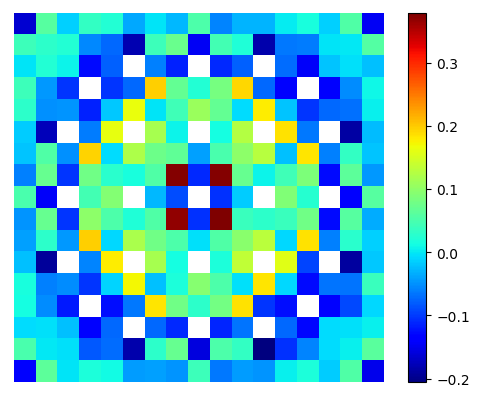
\includegraphics[width=\linewidth]{figures/assembly/fiss-single-step-errors}
  \caption{}
  \label{fig:assm-fiss-single-step-error}
\end{subfigure}%
\begin{subfigure}{0.45\textwidth}
  \centering
  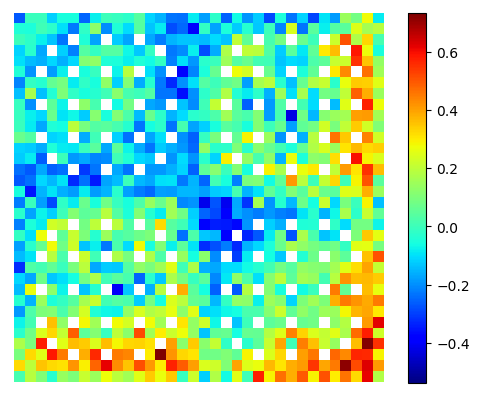
\includegraphics[width=\linewidth]{figures/colorset/fiss-single-step-errors}
  \caption{}
  \label{fig:colorset-fiss-single-step-error}
\end{subfigure}
\caption{OpenMOC fission rate percent relative errors for the assembly (a) and colorset (b) benchmarks.}
\label{fig:fiss-errors}
\end{figure*}

%%%%%%%%%%%%%%%%%%%%%%%%%%%%%%%%%%%%%%%%%%%%%%%%%%%%%%%%%%%%%%%%%%%%%%%%%%%%%%%
\section{Conclusions}
\label{sec:conclusions}
%%%%%%%%%%%%%%%%%%%%%%%%%%%%%%%%%%%%%%%%%%%%%%%%%%%%%%%%%%%%%%%%%%%%%%%%%%%%%%%

Monte Carlo methods are increasingly used to generate multigroup cross sections for coarse mesh neutron diffusion codes. This paper introduced the \texttt{openmc.mgxs} Python module to generate MGXS with the OpenMC Monte Carlo code for neutron transport applications. This new module utilizes OpenMC's tally system to perform stochastic integration of reaction rates and fluxes for a user-specified energy group discretization and spatial mesh. The different types of MGXS computable to date---including standard group-wise constants, as well as prompt and delayed constants---were tabulated here. The \texttt{openmc.mgxs} module leverages OpenMC's Python API, along with its support for tally slicing, merging, and arithmetic, to provide a scalable data-processing framework complementary to but separate from the transport kernel implemented in the OpenMC executable.

A case study used the multigroup OpenMOC transport code with 70-group MGXS generated by OpenMC to model two heterogeneous PWR benchmarks. The study showed that OpenMOC predicted eigenvalues to within 50 pcm and fission rates to within 1\% of reference solutions computed by OpenMC, demonstrating the efficacy of the \texttt{openmc.mgxs} module to enable highly accurate multigroup transport calculations. \textcolor{red}{The multi-group constants generated by OpenMC are intended for use by fine-mesh transport rather than coarse-mesh diffusion codes, which brings its own set of unique -- though not mutually exclusive -- challenges with respect to few-group diffusion.} We expect that \texttt{openmc.mgxs} may prove to be a useful platform for research to address these challenges for MC-based MGXS generation in the future.

%A fine spatial and/or energy discretization may be used by OpenMC to tabulate MGXS, and subsequently condensed in energy and/or homogenized in space with data processing features in Python.

%%%%%%%%%%%%%%%%%%%%%%%%%%%%%%%%%%%%%%%%%%%%%%%%%%%%%%%%%%%%%%%%%%%%%%%%%%%%%%%
\section*{Acknowledgments}
%%%%%%%%%%%%%%%%%%%%%%%%%%%%%%%%%%%%%%%%%%%%%%%%%%%%%%%%%%%%%%%%%%%%%%%%%%%%%%%


%\section*{References}
\setlength{\baselineskip}{12pt}
\bibliography{references}
\bibliographystyle{ans}

\end{document}
